\documentclass[11pt]{article}

    \usepackage[breakable]{tcolorbox}
    \usepackage{parskip} % Stop auto-indenting (to mimic markdown behaviour)
    \usepackage{pdfpages}
    \usepackage{iftex}
    \ifPDFTeX
    	\usepackage[T1]{fontenc}
    	\usepackage{mathpazo}
    \else
    	\usepackage{fontspec}
    \fi

    % Basic figure setup, for now with no caption control since it's done
    % automatically by Pandoc (which extracts ![](path) syntax from Markdown).
    \usepackage{graphicx}
    % Maintain compatibility with old templates. Remove in nbconvert 6.0
    \let\Oldincludegraphics\includegraphics
    % Ensure that by default, figures have no caption (until we provide a
    % proper Figure object with a Caption API and a way to capture that
    % in the conversion process - todo).
    \usepackage{caption}
    \DeclareCaptionFormat{nocaption}{}
    \captionsetup{format=nocaption,aboveskip=0pt,belowskip=0pt}

    \usepackage[Export]{adjustbox} % Used to constrain images to a maximum size
    \adjustboxset{max size={0.9\linewidth}{0.9\paperheight}}
    \usepackage{float}
    \floatplacement{figure}{H} % forces figures to be placed at the correct location
    \usepackage{xcolor} % Allow colors to be defined
    \usepackage{enumerate} % Needed for markdown enumerations to work
    \usepackage{geometry} % Used to adjust the document margins
    \usepackage{amsmath} % Equations
    \usepackage{amssymb} % Equations
    \usepackage{textcomp} % defines textquotesingle
    % Hack from http://tex.stackexchange.com/a/47451/13684:
    \AtBeginDocument{%
        \def\PYZsq{\textquotesingle}% Upright quotes in Pygmentized code
    }
    \usepackage{upquote} % Upright quotes for verbatim code
    \usepackage{eurosym} % defines \euro
    \usepackage[mathletters]{ucs} % Extended unicode (utf-8) support
    \usepackage{fancyvrb} % verbatim replacement that allows latex
    \usepackage{grffile} % extends the file name processing of package graphics 
                         % to support a larger range
    \makeatletter % fix for grffile with XeLaTeX
    \def\Gread@@xetex#1{%
      \IfFileExists{"\Gin@base".bb}%
      {\Gread@eps{\Gin@base.bb}}%
      {\Gread@@xetex@aux#1}%
    }
    \makeatother

    % The hyperref package gives us a pdf with properly built
    % internal navigation ('pdf bookmarks' for the table of contents,
    % internal cross-reference links, web links for URLs, etc.)
    \usepackage{hyperref}
    % The default LaTeX title has an obnoxious amount of whitespace. By default,
    % titling removes some of it. It also provides customization options.
    \usepackage{titling}
    \usepackage{longtable} % longtable support required by pandoc >1.10
    \usepackage{booktabs}  % table support for pandoc > 1.12.2
    \usepackage[inline]{enumitem} % IRkernel/repr support (it uses the enumerate* environment)
    \usepackage[normalem]{ulem} % ulem is needed to support strikethroughs (\sout)
                                % normalem makes italics be italics, not underlines
    \usepackage{mathrsfs}
    

    
    % Colors for the hyperref package
    \definecolor{urlcolor}{rgb}{0,.145,.698}
    \definecolor{linkcolor}{rgb}{.71,0.21,0.01}
    \definecolor{citecolor}{rgb}{.12,.54,.11}

    % ANSI colors
    \definecolor{ansi-black}{HTML}{3E424D}
    \definecolor{ansi-black-intense}{HTML}{282C36}
    \definecolor{ansi-red}{HTML}{E75C58}
    \definecolor{ansi-red-intense}{HTML}{B22B31}
    \definecolor{ansi-green}{HTML}{00A250}
    \definecolor{ansi-green-intense}{HTML}{007427}
    \definecolor{ansi-yellow}{HTML}{DDB62B}
    \definecolor{ansi-yellow-intense}{HTML}{B27D12}
    \definecolor{ansi-blue}{HTML}{208FFB}
    \definecolor{ansi-blue-intense}{HTML}{0065CA}
    \definecolor{ansi-magenta}{HTML}{D160C4}
    \definecolor{ansi-magenta-intense}{HTML}{A03196}
    \definecolor{ansi-cyan}{HTML}{60C6C8}
    \definecolor{ansi-cyan-intense}{HTML}{258F8F}
    \definecolor{ansi-white}{HTML}{C5C1B4}
    \definecolor{ansi-white-intense}{HTML}{A1A6B2}
    \definecolor{ansi-default-inverse-fg}{HTML}{FFFFFF}
    \definecolor{ansi-default-inverse-bg}{HTML}{000000}

    % commands and environments needed by pandoc snippets
    % extracted from the output of `pandoc -s`
    \providecommand{\tightlist}{%
      \setlength{\itemsep}{0pt}\setlength{\parskip}{0pt}}
    \DefineVerbatimEnvironment{Highlighting}{Verbatim}{commandchars=\\\{\}}
    % Add ',fontsize=\small' for more characters per line
    \newenvironment{Shaded}{}{}
    \newcommand{\KeywordTok}[1]{\textcolor[rgb]{0.00,0.44,0.13}{\textbf{{#1}}}}
    \newcommand{\DataTypeTok}[1]{\textcolor[rgb]{0.56,0.13,0.00}{{#1}}}
    \newcommand{\DecValTok}[1]{\textcolor[rgb]{0.25,0.63,0.44}{{#1}}}
    \newcommand{\BaseNTok}[1]{\textcolor[rgb]{0.25,0.63,0.44}{{#1}}}
    \newcommand{\FloatTok}[1]{\textcolor[rgb]{0.25,0.63,0.44}{{#1}}}
    \newcommand{\CharTok}[1]{\textcolor[rgb]{0.25,0.44,0.63}{{#1}}}
    \newcommand{\StringTok}[1]{\textcolor[rgb]{0.25,0.44,0.63}{{#1}}}
    \newcommand{\CommentTok}[1]{\textcolor[rgb]{0.38,0.63,0.69}{\textit{{#1}}}}
    \newcommand{\OtherTok}[1]{\textcolor[rgb]{0.00,0.44,0.13}{{#1}}}
    \newcommand{\AlertTok}[1]{\textcolor[rgb]{1.00,0.00,0.00}{\textbf{{#1}}}}
    \newcommand{\FunctionTok}[1]{\textcolor[rgb]{0.02,0.16,0.49}{{#1}}}
    \newcommand{\RegionMarkerTok}[1]{{#1}}
    \newcommand{\ErrorTok}[1]{\textcolor[rgb]{1.00,0.00,0.00}{\textbf{{#1}}}}
    \newcommand{\NormalTok}[1]{{#1}}
    
    % Additional commands for more recent versions of Pandoc
    \newcommand{\ConstantTok}[1]{\textcolor[rgb]{0.53,0.00,0.00}{{#1}}}
    \newcommand{\SpecialCharTok}[1]{\textcolor[rgb]{0.25,0.44,0.63}{{#1}}}
    \newcommand{\VerbatimStringTok}[1]{\textcolor[rgb]{0.25,0.44,0.63}{{#1}}}
    \newcommand{\SpecialStringTok}[1]{\textcolor[rgb]{0.73,0.40,0.53}{{#1}}}
    \newcommand{\ImportTok}[1]{{#1}}
    \newcommand{\DocumentationTok}[1]{\textcolor[rgb]{0.73,0.13,0.13}{\textit{{#1}}}}
    \newcommand{\AnnotationTok}[1]{\textcolor[rgb]{0.38,0.63,0.69}{\textbf{\textit{{#1}}}}}
    \newcommand{\CommentVarTok}[1]{\textcolor[rgb]{0.38,0.63,0.69}{\textbf{\textit{{#1}}}}}
    \newcommand{\VariableTok}[1]{\textcolor[rgb]{0.10,0.09,0.49}{{#1}}}
    \newcommand{\ControlFlowTok}[1]{\textcolor[rgb]{0.00,0.44,0.13}{\textbf{{#1}}}}
    \newcommand{\OperatorTok}[1]{\textcolor[rgb]{0.40,0.40,0.40}{{#1}}}
    \newcommand{\BuiltInTok}[1]{{#1}}
    \newcommand{\ExtensionTok}[1]{{#1}}
    \newcommand{\PreprocessorTok}[1]{\textcolor[rgb]{0.74,0.48,0.00}{{#1}}}
    \newcommand{\AttributeTok}[1]{\textcolor[rgb]{0.49,0.56,0.16}{{#1}}}
    \newcommand{\InformationTok}[1]{\textcolor[rgb]{0.38,0.63,0.69}{\textbf{\textit{{#1}}}}}
    \newcommand{\WarningTok}[1]{\textcolor[rgb]{0.38,0.63,0.69}{\textbf{\textit{{#1}}}}}
    
    
    % Define a nice break command that doesn't care if a line doesn't already
    % exist.
    \def\br{\hspace*{\fill} \\* }
    % Math Jax compatibility definitions
    \def\gt{>}
    \def\lt{<}
    \let\Oldtex\TeX
    \let\Oldlatex\LaTeX
    \renewcommand{\TeX}{\textrm{\Oldtex}}
    \renewcommand{\LaTeX}{\textrm{\Oldlatex}}
    % Document parameters
    % Document title
    \title{ComS574\_HW3\_sol}
    
    
    
    
    
% Pygments definitions
\makeatletter
\def\PY@reset{\let\PY@it=\relax \let\PY@bf=\relax%
    \let\PY@ul=\relax \let\PY@tc=\relax%
    \let\PY@bc=\relax \let\PY@ff=\relax}
\def\PY@tok#1{\csname PY@tok@#1\endcsname}
\def\PY@toks#1+{\ifx\relax#1\empty\else%
    \PY@tok{#1}\expandafter\PY@toks\fi}
\def\PY@do#1{\PY@bc{\PY@tc{\PY@ul{%
    \PY@it{\PY@bf{\PY@ff{#1}}}}}}}
\def\PY#1#2{\PY@reset\PY@toks#1+\relax+\PY@do{#2}}

\expandafter\def\csname PY@tok@w\endcsname{\def\PY@tc##1{\textcolor[rgb]{0.73,0.73,0.73}{##1}}}
\expandafter\def\csname PY@tok@c\endcsname{\let\PY@it=\textit\def\PY@tc##1{\textcolor[rgb]{0.25,0.50,0.50}{##1}}}
\expandafter\def\csname PY@tok@cp\endcsname{\def\PY@tc##1{\textcolor[rgb]{0.74,0.48,0.00}{##1}}}
\expandafter\def\csname PY@tok@k\endcsname{\let\PY@bf=\textbf\def\PY@tc##1{\textcolor[rgb]{0.00,0.50,0.00}{##1}}}
\expandafter\def\csname PY@tok@kp\endcsname{\def\PY@tc##1{\textcolor[rgb]{0.00,0.50,0.00}{##1}}}
\expandafter\def\csname PY@tok@kt\endcsname{\def\PY@tc##1{\textcolor[rgb]{0.69,0.00,0.25}{##1}}}
\expandafter\def\csname PY@tok@o\endcsname{\def\PY@tc##1{\textcolor[rgb]{0.40,0.40,0.40}{##1}}}
\expandafter\def\csname PY@tok@ow\endcsname{\let\PY@bf=\textbf\def\PY@tc##1{\textcolor[rgb]{0.67,0.13,1.00}{##1}}}
\expandafter\def\csname PY@tok@nb\endcsname{\def\PY@tc##1{\textcolor[rgb]{0.00,0.50,0.00}{##1}}}
\expandafter\def\csname PY@tok@nf\endcsname{\def\PY@tc##1{\textcolor[rgb]{0.00,0.00,1.00}{##1}}}
\expandafter\def\csname PY@tok@nc\endcsname{\let\PY@bf=\textbf\def\PY@tc##1{\textcolor[rgb]{0.00,0.00,1.00}{##1}}}
\expandafter\def\csname PY@tok@nn\endcsname{\let\PY@bf=\textbf\def\PY@tc##1{\textcolor[rgb]{0.00,0.00,1.00}{##1}}}
\expandafter\def\csname PY@tok@ne\endcsname{\let\PY@bf=\textbf\def\PY@tc##1{\textcolor[rgb]{0.82,0.25,0.23}{##1}}}
\expandafter\def\csname PY@tok@nv\endcsname{\def\PY@tc##1{\textcolor[rgb]{0.10,0.09,0.49}{##1}}}
\expandafter\def\csname PY@tok@no\endcsname{\def\PY@tc##1{\textcolor[rgb]{0.53,0.00,0.00}{##1}}}
\expandafter\def\csname PY@tok@nl\endcsname{\def\PY@tc##1{\textcolor[rgb]{0.63,0.63,0.00}{##1}}}
\expandafter\def\csname PY@tok@ni\endcsname{\let\PY@bf=\textbf\def\PY@tc##1{\textcolor[rgb]{0.60,0.60,0.60}{##1}}}
\expandafter\def\csname PY@tok@na\endcsname{\def\PY@tc##1{\textcolor[rgb]{0.49,0.56,0.16}{##1}}}
\expandafter\def\csname PY@tok@nt\endcsname{\let\PY@bf=\textbf\def\PY@tc##1{\textcolor[rgb]{0.00,0.50,0.00}{##1}}}
\expandafter\def\csname PY@tok@nd\endcsname{\def\PY@tc##1{\textcolor[rgb]{0.67,0.13,1.00}{##1}}}
\expandafter\def\csname PY@tok@s\endcsname{\def\PY@tc##1{\textcolor[rgb]{0.73,0.13,0.13}{##1}}}
\expandafter\def\csname PY@tok@sd\endcsname{\let\PY@it=\textit\def\PY@tc##1{\textcolor[rgb]{0.73,0.13,0.13}{##1}}}
\expandafter\def\csname PY@tok@si\endcsname{\let\PY@bf=\textbf\def\PY@tc##1{\textcolor[rgb]{0.73,0.40,0.53}{##1}}}
\expandafter\def\csname PY@tok@se\endcsname{\let\PY@bf=\textbf\def\PY@tc##1{\textcolor[rgb]{0.73,0.40,0.13}{##1}}}
\expandafter\def\csname PY@tok@sr\endcsname{\def\PY@tc##1{\textcolor[rgb]{0.73,0.40,0.53}{##1}}}
\expandafter\def\csname PY@tok@ss\endcsname{\def\PY@tc##1{\textcolor[rgb]{0.10,0.09,0.49}{##1}}}
\expandafter\def\csname PY@tok@sx\endcsname{\def\PY@tc##1{\textcolor[rgb]{0.00,0.50,0.00}{##1}}}
\expandafter\def\csname PY@tok@m\endcsname{\def\PY@tc##1{\textcolor[rgb]{0.40,0.40,0.40}{##1}}}
\expandafter\def\csname PY@tok@gh\endcsname{\let\PY@bf=\textbf\def\PY@tc##1{\textcolor[rgb]{0.00,0.00,0.50}{##1}}}
\expandafter\def\csname PY@tok@gu\endcsname{\let\PY@bf=\textbf\def\PY@tc##1{\textcolor[rgb]{0.50,0.00,0.50}{##1}}}
\expandafter\def\csname PY@tok@gd\endcsname{\def\PY@tc##1{\textcolor[rgb]{0.63,0.00,0.00}{##1}}}
\expandafter\def\csname PY@tok@gi\endcsname{\def\PY@tc##1{\textcolor[rgb]{0.00,0.63,0.00}{##1}}}
\expandafter\def\csname PY@tok@gr\endcsname{\def\PY@tc##1{\textcolor[rgb]{1.00,0.00,0.00}{##1}}}
\expandafter\def\csname PY@tok@ge\endcsname{\let\PY@it=\textit}
\expandafter\def\csname PY@tok@gs\endcsname{\let\PY@bf=\textbf}
\expandafter\def\csname PY@tok@gp\endcsname{\let\PY@bf=\textbf\def\PY@tc##1{\textcolor[rgb]{0.00,0.00,0.50}{##1}}}
\expandafter\def\csname PY@tok@go\endcsname{\def\PY@tc##1{\textcolor[rgb]{0.53,0.53,0.53}{##1}}}
\expandafter\def\csname PY@tok@gt\endcsname{\def\PY@tc##1{\textcolor[rgb]{0.00,0.27,0.87}{##1}}}
\expandafter\def\csname PY@tok@err\endcsname{\def\PY@bc##1{\setlength{\fboxsep}{0pt}\fcolorbox[rgb]{1.00,0.00,0.00}{1,1,1}{\strut ##1}}}
\expandafter\def\csname PY@tok@kc\endcsname{\let\PY@bf=\textbf\def\PY@tc##1{\textcolor[rgb]{0.00,0.50,0.00}{##1}}}
\expandafter\def\csname PY@tok@kd\endcsname{\let\PY@bf=\textbf\def\PY@tc##1{\textcolor[rgb]{0.00,0.50,0.00}{##1}}}
\expandafter\def\csname PY@tok@kn\endcsname{\let\PY@bf=\textbf\def\PY@tc##1{\textcolor[rgb]{0.00,0.50,0.00}{##1}}}
\expandafter\def\csname PY@tok@kr\endcsname{\let\PY@bf=\textbf\def\PY@tc##1{\textcolor[rgb]{0.00,0.50,0.00}{##1}}}
\expandafter\def\csname PY@tok@bp\endcsname{\def\PY@tc##1{\textcolor[rgb]{0.00,0.50,0.00}{##1}}}
\expandafter\def\csname PY@tok@fm\endcsname{\def\PY@tc##1{\textcolor[rgb]{0.00,0.00,1.00}{##1}}}
\expandafter\def\csname PY@tok@vc\endcsname{\def\PY@tc##1{\textcolor[rgb]{0.10,0.09,0.49}{##1}}}
\expandafter\def\csname PY@tok@vg\endcsname{\def\PY@tc##1{\textcolor[rgb]{0.10,0.09,0.49}{##1}}}
\expandafter\def\csname PY@tok@vi\endcsname{\def\PY@tc##1{\textcolor[rgb]{0.10,0.09,0.49}{##1}}}
\expandafter\def\csname PY@tok@vm\endcsname{\def\PY@tc##1{\textcolor[rgb]{0.10,0.09,0.49}{##1}}}
\expandafter\def\csname PY@tok@sa\endcsname{\def\PY@tc##1{\textcolor[rgb]{0.73,0.13,0.13}{##1}}}
\expandafter\def\csname PY@tok@sb\endcsname{\def\PY@tc##1{\textcolor[rgb]{0.73,0.13,0.13}{##1}}}
\expandafter\def\csname PY@tok@sc\endcsname{\def\PY@tc##1{\textcolor[rgb]{0.73,0.13,0.13}{##1}}}
\expandafter\def\csname PY@tok@dl\endcsname{\def\PY@tc##1{\textcolor[rgb]{0.73,0.13,0.13}{##1}}}
\expandafter\def\csname PY@tok@s2\endcsname{\def\PY@tc##1{\textcolor[rgb]{0.73,0.13,0.13}{##1}}}
\expandafter\def\csname PY@tok@sh\endcsname{\def\PY@tc##1{\textcolor[rgb]{0.73,0.13,0.13}{##1}}}
\expandafter\def\csname PY@tok@s1\endcsname{\def\PY@tc##1{\textcolor[rgb]{0.73,0.13,0.13}{##1}}}
\expandafter\def\csname PY@tok@mb\endcsname{\def\PY@tc##1{\textcolor[rgb]{0.40,0.40,0.40}{##1}}}
\expandafter\def\csname PY@tok@mf\endcsname{\def\PY@tc##1{\textcolor[rgb]{0.40,0.40,0.40}{##1}}}
\expandafter\def\csname PY@tok@mh\endcsname{\def\PY@tc##1{\textcolor[rgb]{0.40,0.40,0.40}{##1}}}
\expandafter\def\csname PY@tok@mi\endcsname{\def\PY@tc##1{\textcolor[rgb]{0.40,0.40,0.40}{##1}}}
\expandafter\def\csname PY@tok@il\endcsname{\def\PY@tc##1{\textcolor[rgb]{0.40,0.40,0.40}{##1}}}
\expandafter\def\csname PY@tok@mo\endcsname{\def\PY@tc##1{\textcolor[rgb]{0.40,0.40,0.40}{##1}}}
\expandafter\def\csname PY@tok@ch\endcsname{\let\PY@it=\textit\def\PY@tc##1{\textcolor[rgb]{0.25,0.50,0.50}{##1}}}
\expandafter\def\csname PY@tok@cm\endcsname{\let\PY@it=\textit\def\PY@tc##1{\textcolor[rgb]{0.25,0.50,0.50}{##1}}}
\expandafter\def\csname PY@tok@cpf\endcsname{\let\PY@it=\textit\def\PY@tc##1{\textcolor[rgb]{0.25,0.50,0.50}{##1}}}
\expandafter\def\csname PY@tok@c1\endcsname{\let\PY@it=\textit\def\PY@tc##1{\textcolor[rgb]{0.25,0.50,0.50}{##1}}}
\expandafter\def\csname PY@tok@cs\endcsname{\let\PY@it=\textit\def\PY@tc##1{\textcolor[rgb]{0.25,0.50,0.50}{##1}}}

\def\PYZbs{\char`\\}
\def\PYZus{\char`\_}
\def\PYZob{\char`\{}
\def\PYZcb{\char`\}}
\def\PYZca{\char`\^}
\def\PYZam{\char`\&}
\def\PYZlt{\char`\<}
\def\PYZgt{\char`\>}
\def\PYZsh{\char`\#}
\def\PYZpc{\char`\%}
\def\PYZdl{\char`\$}
\def\PYZhy{\char`\-}
\def\PYZsq{\char`\'}
\def\PYZdq{\char`\"}
\def\PYZti{\char`\~}
% for compatibility with earlier versions
\def\PYZat{@}
\def\PYZlb{[}
\def\PYZrb{]}
\makeatother


    % For linebreaks inside Verbatim environment from package fancyvrb. 
    \makeatletter
        \newbox\Wrappedcontinuationbox 
        \newbox\Wrappedvisiblespacebox 
        \newcommand*\Wrappedvisiblespace {\textcolor{red}{\textvisiblespace}} 
        \newcommand*\Wrappedcontinuationsymbol {\textcolor{red}{\llap{\tiny$\m@th\hookrightarrow$}}} 
        \newcommand*\Wrappedcontinuationindent {3ex } 
        \newcommand*\Wrappedafterbreak {\kern\Wrappedcontinuationindent\copy\Wrappedcontinuationbox} 
        % Take advantage of the already applied Pygments mark-up to insert 
        % potential linebreaks for TeX processing. 
        %        {, <, #, %, $, ' and ": go to next line. 
        %        _, }, ^, &, >, - and ~: stay at end of broken line. 
        % Use of \textquotesingle for straight quote. 
        \newcommand*\Wrappedbreaksatspecials {% 
            \def\PYGZus{\discretionary{\char`\_}{\Wrappedafterbreak}{\char`\_}}% 
            \def\PYGZob{\discretionary{}{\Wrappedafterbreak\char`\{}{\char`\{}}% 
            \def\PYGZcb{\discretionary{\char`\}}{\Wrappedafterbreak}{\char`\}}}% 
            \def\PYGZca{\discretionary{\char`\^}{\Wrappedafterbreak}{\char`\^}}% 
            \def\PYGZam{\discretionary{\char`\&}{\Wrappedafterbreak}{\char`\&}}% 
            \def\PYGZlt{\discretionary{}{\Wrappedafterbreak\char`\<}{\char`\<}}% 
            \def\PYGZgt{\discretionary{\char`\>}{\Wrappedafterbreak}{\char`\>}}% 
            \def\PYGZsh{\discretionary{}{\Wrappedafterbreak\char`\#}{\char`\#}}% 
            \def\PYGZpc{\discretionary{}{\Wrappedafterbreak\char`\%}{\char`\%}}% 
            \def\PYGZdl{\discretionary{}{\Wrappedafterbreak\char`\$}{\char`\$}}% 
            \def\PYGZhy{\discretionary{\char`\-}{\Wrappedafterbreak}{\char`\-}}% 
            \def\PYGZsq{\discretionary{}{\Wrappedafterbreak\textquotesingle}{\textquotesingle}}% 
            \def\PYGZdq{\discretionary{}{\Wrappedafterbreak\char`\"}{\char`\"}}% 
            \def\PYGZti{\discretionary{\char`\~}{\Wrappedafterbreak}{\char`\~}}% 
        } 
        % Some characters . , ; ? ! / are not pygmentized. 
        % This macro makes them "active" and they will insert potential linebreaks 
        \newcommand*\Wrappedbreaksatpunct {% 
            \lccode`\~`\.\lowercase{\def~}{\discretionary{\hbox{\char`\.}}{\Wrappedafterbreak}{\hbox{\char`\.}}}% 
            \lccode`\~`\,\lowercase{\def~}{\discretionary{\hbox{\char`\,}}{\Wrappedafterbreak}{\hbox{\char`\,}}}% 
            \lccode`\~`\;\lowercase{\def~}{\discretionary{\hbox{\char`\;}}{\Wrappedafterbreak}{\hbox{\char`\;}}}% 
            \lccode`\~`\:\lowercase{\def~}{\discretionary{\hbox{\char`\:}}{\Wrappedafterbreak}{\hbox{\char`\:}}}% 
            \lccode`\~`\?\lowercase{\def~}{\discretionary{\hbox{\char`\?}}{\Wrappedafterbreak}{\hbox{\char`\?}}}% 
            \lccode`\~`\!\lowercase{\def~}{\discretionary{\hbox{\char`\!}}{\Wrappedafterbreak}{\hbox{\char`\!}}}% 
            \lccode`\~`\/\lowercase{\def~}{\discretionary{\hbox{\char`\/}}{\Wrappedafterbreak}{\hbox{\char`\/}}}% 
            \catcode`\.\active
            \catcode`\,\active 
            \catcode`\;\active
            \catcode`\:\active
            \catcode`\?\active
            \catcode`\!\active
            \catcode`\/\active 
            \lccode`\~`\~ 	
        }
    \makeatother

    \let\OriginalVerbatim=\Verbatim
    \makeatletter
    \renewcommand{\Verbatim}[1][1]{%
        %\parskip\z@skip
        \sbox\Wrappedcontinuationbox {\Wrappedcontinuationsymbol}%
        \sbox\Wrappedvisiblespacebox {\FV@SetupFont\Wrappedvisiblespace}%
        \def\FancyVerbFormatLine ##1{\hsize\linewidth
            \vtop{\raggedright\hyphenpenalty\z@\exhyphenpenalty\z@
                \doublehyphendemerits\z@\finalhyphendemerits\z@
                \strut ##1\strut}%
        }%
        % If the linebreak is at a space, the latter will be displayed as visible
        % space at end of first line, and a continuation symbol starts next line.
        % Stretch/shrink are however usually zero for typewriter font.
        \def\FV@Space {%
            \nobreak\hskip\z@ plus\fontdimen3\font minus\fontdimen4\font
            \discretionary{\copy\Wrappedvisiblespacebox}{\Wrappedafterbreak}
            {\kern\fontdimen2\font}%
        }%
        
        % Allow breaks at special characters using \PYG... macros.
        \Wrappedbreaksatspecials
        % Breaks at punctuation characters . , ; ? ! and / need catcode=\active 	
        \OriginalVerbatim[#1,codes*=\Wrappedbreaksatpunct]%
    }
    \makeatother

    % Exact colors from NB
    \definecolor{incolor}{HTML}{303F9F}
    \definecolor{outcolor}{HTML}{D84315}
    \definecolor{cellborder}{HTML}{CFCFCF}
    \definecolor{cellbackground}{HTML}{F7F7F7}
    
    % prompt
    \makeatletter
    \newcommand{\boxspacing}{\kern\kvtcb@left@rule\kern\kvtcb@boxsep}
    \makeatother
    \newcommand{\prompt}[4]{
        \ttfamily\llap{{\color{#2}[#3]:\hspace{3pt}#4}}\vspace{-\baselineskip}
    }
    

    
    % Prevent overflowing lines due to hard-to-break entities
    \sloppy 
    % Setup hyperref package
    \hypersetup{
      breaklinks=true,  % so long urls are correctly broken across lines
      colorlinks=true,
      urlcolor=urlcolor,
      linkcolor=linkcolor,
      citecolor=citecolor,
      }
    % Slightly bigger margins than the latex defaults
    
    \geometry{verbose,tmargin=1in,bmargin=1in,lmargin=1in,rmargin=1in}
    
    

\begin{document}
    
    \maketitle
    
    

    
    ComS 574

HW 3

Kanak Choudhury

    \hypertarget{problem-1-2}{%
\section{Problem 1 \& 2:}\label{problem-1-2}}

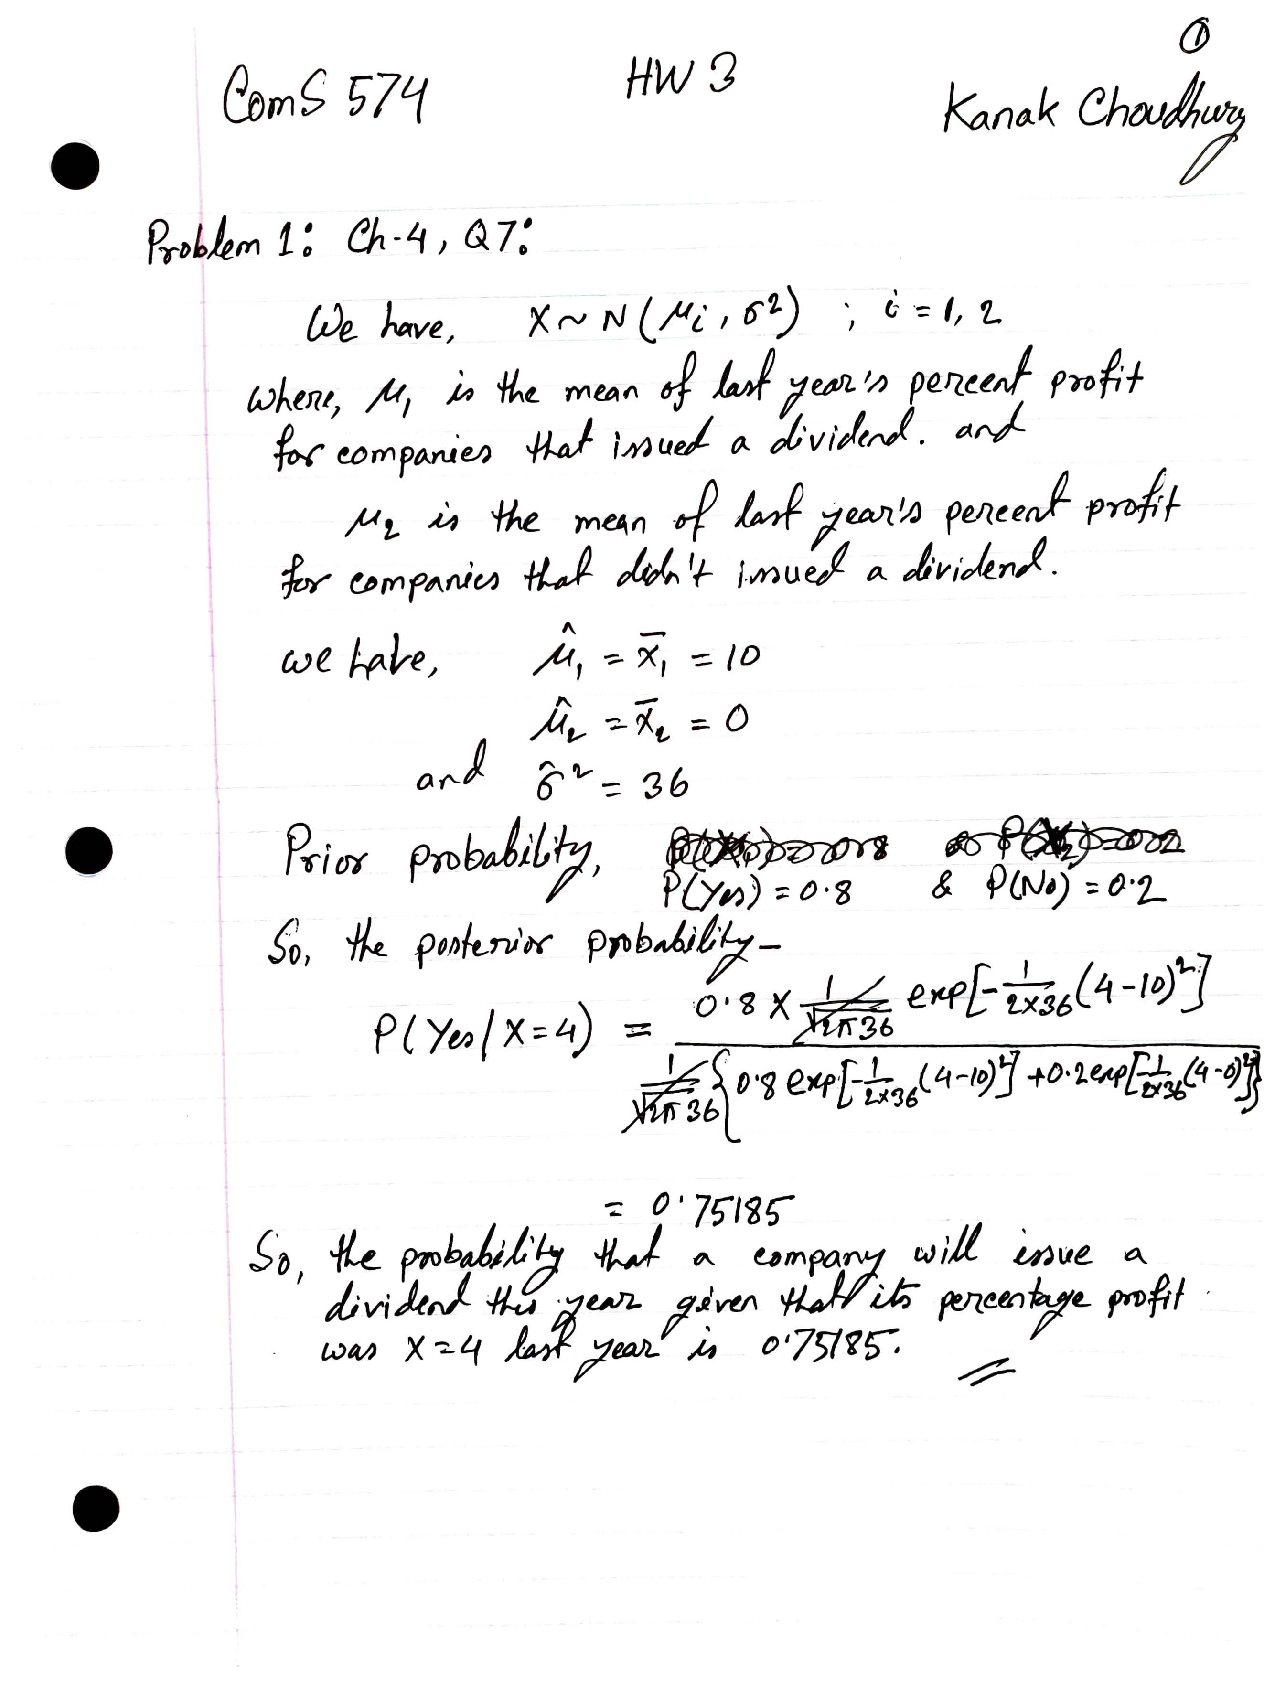
\includepdf[pages=-]{D:/ISU/COMS 574 - Introduction to Machine Learning/HW/HW3/ComS_574_HW3_1-2.pdf}

    \hypertarget{problem-3-ch-9-1}{%
\section{Problem 3: Ch 9 \#1}\label{problem-3-ch-9-1}}

    \hypertarget{a}{%
\subsection{(a)}\label{a}}

Sketch the hyperplane \(1 + 3X_1 - X_2 = 0\). Indicate the set of points
for which \(1 + 3X_1 - X_2 > 0\), as well as the set of points for which
\(1 + 3X_1 - X_2 < 0\).

\hypertarget{b}{%
\subsection{(b)}\label{b}}

On the same plot, sketch the hyperplane \(-2 + X_1 + 2X_2 = 0\).
Indicate the set of points for which \(-2+ X_1 +2X_2 > 0\), as well as
the set of points for which \(-2+ X_1 + 2X_2 < 0\).

    \begin{tcolorbox}[breakable, size=fbox, boxrule=1pt, pad at break*=1mm,colback=cellbackground, colframe=cellborder]
\prompt{In}{incolor}{368}{\boxspacing}
\begin{Verbatim}[commandchars=\\\{\}]
\PY{k+kn}{import} \PY{n+nn}{numpy} \PY{k}{as} \PY{n+nn}{np}
\PY{k+kn}{from} \PY{n+nn}{matplotlib} \PY{k}{import} \PY{n}{pyplot} \PY{k}{as} \PY{n}{plt}
\PY{k+kn}{import} \PY{n+nn}{turtle}
\end{Verbatim}
\end{tcolorbox}

    \begin{tcolorbox}[breakable, size=fbox, boxrule=1pt, pad at break*=1mm,colback=cellbackground, colframe=cellborder]
\prompt{In}{incolor}{369}{\boxspacing}
\begin{Verbatim}[commandchars=\\\{\}]
\PY{n}{x1} \PY{o}{=} \PY{n}{np}\PY{o}{.}\PY{n}{linspace}\PY{p}{(}\PY{o}{\PYZhy{}}\PY{l+m+mi}{100}\PY{p}{,} \PY{l+m+mi}{100}\PY{p}{,} \PY{l+m+mi}{50000}\PY{p}{)}
\PY{n}{x2} \PY{o}{=} \PY{l+m+mi}{1}\PY{o}{+}\PY{l+m+mi}{3}\PY{o}{*}\PY{n}{x1}
\PY{n}{x22} \PY{o}{=} \PY{n}{np}\PY{o}{.}\PY{n}{random}\PY{o}{.}\PY{n}{uniform}\PY{p}{(}\PY{l+m+mi}{301}\PY{p}{,} \PY{o}{\PYZhy{}}\PY{l+m+mi}{301}\PY{p}{,} \PY{l+m+mi}{50000}\PY{p}{)}
\PY{n}{x2b} \PY{o}{=} \PY{l+m+mi}{1}\PY{o}{\PYZhy{}}\PY{n}{x1}\PY{o}{/}\PY{l+m+mi}{2}

\PY{n}{plt}\PY{o}{.}\PY{n}{plot}\PY{p}{(}\PY{n}{x1}\PY{p}{,} \PY{n}{x2}\PY{p}{,} \PY{n}{linewidth}\PY{o}{=}\PY{l+m+mi}{5}\PY{p}{,} \PY{n}{color} \PY{o}{=} \PY{l+s+s1}{\PYZsq{}}\PY{l+s+s1}{red}\PY{l+s+s1}{\PYZsq{}}\PY{p}{,} \PY{n}{label} \PY{o}{=} \PY{l+s+s1}{\PYZsq{}}\PY{l+s+s1}{\PYZdl{}1 + 3X\PYZus{}1 - X\PYZus{}2=0\PYZdl{}}\PY{l+s+s1}{\PYZsq{}}\PY{p}{)}
\PY{n}{plt}\PY{o}{.}\PY{n}{plot}\PY{p}{(}\PY{n}{x1}\PY{p}{,} \PY{n}{x2b}\PY{p}{,} \PY{n}{linewidth}\PY{o}{=}\PY{l+m+mi}{5}\PY{p}{,} \PY{n}{color} \PY{o}{=} \PY{l+s+s1}{\PYZsq{}}\PY{l+s+s1}{green}\PY{l+s+s1}{\PYZsq{}}\PY{p}{,} \PY{n}{label} \PY{o}{=} \PY{l+s+s1}{\PYZsq{}}\PY{l+s+s1}{\PYZdl{}-2+ X\PYZus{}1 +2X\PYZus{}2 = 0\PYZdl{}}\PY{l+s+s1}{\PYZsq{}}\PY{p}{)}

\PY{n}{plt}\PY{o}{.}\PY{n}{fill\PYZus{}between}\PY{p}{(}\PY{n}{x1}\PY{p}{,} \PY{n}{x2}\PY{p}{,} \PY{n}{x22}\PY{p}{,} \PY{n}{where}\PY{o}{=}\PY{n}{x22}\PY{o}{\PYZgt{}}\PY{n}{x2}\PY{p}{,}  \PY{n}{alpha} \PY{o}{=} \PY{l+m+mi}{1}\PY{p}{)}
\PY{n}{plt}\PY{o}{.}\PY{n}{fill\PYZus{}between}\PY{p}{(}\PY{n}{x1}\PY{p}{,} \PY{n}{x2}\PY{p}{,} \PY{n}{x22}\PY{p}{,} \PY{n}{where}\PY{o}{=}\PY{n}{x22}\PY{o}{\PYZlt{}}\PY{n}{x2}\PY{p}{,}  \PY{n}{alpha} \PY{o}{=} \PY{l+m+mi}{1}\PY{p}{)}

\PY{n}{plt}\PY{o}{.}\PY{n}{fill\PYZus{}between}\PY{p}{(}\PY{n}{x1}\PY{p}{,} \PY{n}{x2b}\PY{p}{,} \PY{n}{x22}\PY{p}{,} \PY{n}{where}\PY{o}{=}\PY{n}{x22}\PY{o}{\PYZgt{}}\PY{n}{x2b}\PY{p}{,}  \PY{n}{alpha} \PY{o}{=} \PY{l+m+mi}{1}\PY{p}{)}
\PY{n}{plt}\PY{o}{.}\PY{n}{fill\PYZus{}between}\PY{p}{(}\PY{n}{x1}\PY{p}{,} \PY{n}{x2b}\PY{p}{,} \PY{n}{x22}\PY{p}{,} \PY{n}{where}\PY{o}{=}\PY{n}{x22}\PY{o}{\PYZlt{}}\PY{n}{x2b}\PY{p}{,}  \PY{n}{alpha} \PY{o}{=} \PY{l+m+mi}{1}\PY{p}{)}

\PY{n}{plt}\PY{o}{.}\PY{n}{text}\PY{p}{(}\PY{o}{\PYZhy{}}\PY{l+m+mi}{75}\PY{p}{,} \PY{l+m+mi}{120}\PY{p}{,} \PY{l+s+s1}{\PYZsq{}}\PY{l+s+s1}{\PYZdl{}1 + 3X\PYZus{}1 - X\PYZus{}2 \PYZlt{} 0\PYZdl{}}\PY{l+s+s1}{\PYZsq{}}\PY{p}{,} \PY{n}{color} \PY{o}{=} \PY{l+s+s1}{\PYZsq{}}\PY{l+s+s1}{red}\PY{l+s+s1}{\PYZsq{}}\PY{p}{)}
\PY{n}{plt}\PY{o}{.}\PY{n}{text}\PY{p}{(}\PY{l+m+mi}{5}\PY{p}{,} \PY{o}{\PYZhy{}}\PY{l+m+mi}{200}\PY{p}{,} \PY{l+s+s1}{\PYZsq{}}\PY{l+s+s1}{\PYZdl{}1 + 3X\PYZus{}1 - X\PYZus{}2 \PYZgt{} 0\PYZdl{}}\PY{l+s+s1}{\PYZsq{}}\PY{p}{,} \PY{n}{color} \PY{o}{=} \PY{l+s+s1}{\PYZsq{}}\PY{l+s+s1}{red}\PY{l+s+s1}{\PYZsq{}}\PY{p}{)}
\PY{n}{plt}\PY{o}{.}\PY{n}{text}\PY{p}{(}\PY{l+m+mi}{40}\PY{p}{,} \PY{l+m+mi}{70}\PY{p}{,} \PY{l+s+s1}{\PYZsq{}}\PY{l+s+s1}{\PYZdl{}1 + 3X\PYZus{}1 - X\PYZus{}2 \PYZgt{} 0\PYZdl{}}\PY{l+s+s1}{\PYZsq{}}\PY{p}{,} \PY{n}{color} \PY{o}{=} \PY{l+s+s1}{\PYZsq{}}\PY{l+s+s1}{red}\PY{l+s+s1}{\PYZsq{}}\PY{p}{)}
\PY{n}{plt}\PY{o}{.}\PY{n}{text}\PY{p}{(}\PY{o}{\PYZhy{}}\PY{l+m+mi}{90}\PY{p}{,} \PY{o}{\PYZhy{}}\PY{l+m+mi}{20}\PY{p}{,} \PY{l+s+s1}{\PYZsq{}}\PY{l+s+s1}{\PYZdl{}1 + 3X\PYZus{}1 - X\PYZus{}2 \PYZlt{} 0\PYZdl{}}\PY{l+s+s1}{\PYZsq{}}\PY{p}{,} \PY{n}{color} \PY{o}{=} \PY{l+s+s1}{\PYZsq{}}\PY{l+s+s1}{red}\PY{l+s+s1}{\PYZsq{}}\PY{p}{)}

\PY{n}{plt}\PY{o}{.}\PY{n}{text}\PY{p}{(}\PY{o}{\PYZhy{}}\PY{l+m+mi}{75}\PY{p}{,} \PY{l+m+mi}{70}\PY{p}{,} \PY{l+s+s1}{\PYZsq{}}\PY{l+s+s1}{\PYZdl{}-2+ X\PYZus{}1 +2X\PYZus{}2 \PYZgt{} 0\PYZdl{}}\PY{l+s+s1}{\PYZsq{}}\PY{p}{,} \PY{n}{color} \PY{o}{=} \PY{l+s+s1}{\PYZsq{}}\PY{l+s+s1}{green}\PY{l+s+s1}{\PYZsq{}}\PY{p}{)}
\PY{n}{plt}\PY{o}{.}\PY{n}{text}\PY{p}{(}\PY{l+m+mi}{5}\PY{p}{,} \PY{o}{\PYZhy{}}\PY{l+m+mi}{250}\PY{p}{,} \PY{l+s+s1}{\PYZsq{}}\PY{l+s+s1}{\PYZdl{}-2+ X\PYZus{}1 +2X\PYZus{}2 \PYZlt{} 0\PYZdl{}}\PY{l+s+s1}{\PYZsq{}}\PY{p}{,} \PY{n}{color} \PY{o}{=} \PY{l+s+s1}{\PYZsq{}}\PY{l+s+s1}{green}\PY{l+s+s1}{\PYZsq{}}\PY{p}{)}
\PY{n}{plt}\PY{o}{.}\PY{n}{text}\PY{p}{(}\PY{l+m+mi}{30}\PY{p}{,} \PY{l+m+mi}{20}\PY{p}{,} \PY{l+s+s1}{\PYZsq{}}\PY{l+s+s1}{\PYZdl{}-2+ X\PYZus{}1 +2X\PYZus{}2 \PYZgt{} 0\PYZdl{}}\PY{l+s+s1}{\PYZsq{}}\PY{p}{,} \PY{n}{color} \PY{o}{=} \PY{l+s+s1}{\PYZsq{}}\PY{l+s+s1}{green}\PY{l+s+s1}{\PYZsq{}}\PY{p}{)}
\PY{n}{plt}\PY{o}{.}\PY{n}{text}\PY{p}{(}\PY{o}{\PYZhy{}}\PY{l+m+mi}{90}\PY{p}{,} \PY{o}{\PYZhy{}}\PY{l+m+mi}{80}\PY{p}{,} \PY{l+s+s1}{\PYZsq{}}\PY{l+s+s1}{\PYZdl{}-2+ X\PYZus{}1 +2X\PYZus{}2 \PYZlt{} 0\PYZdl{}}\PY{l+s+s1}{\PYZsq{}}\PY{p}{,} \PY{n}{color} \PY{o}{=} \PY{l+s+s1}{\PYZsq{}}\PY{l+s+s1}{green}\PY{l+s+s1}{\PYZsq{}}\PY{p}{)}
\PY{n}{plt}\PY{o}{.}\PY{n}{legend}\PY{p}{(}\PY{n}{loc} \PY{o}{=} \PY{l+s+s1}{\PYZsq{}}\PY{l+s+s1}{upper left}\PY{l+s+s1}{\PYZsq{}}\PY{p}{,} \PY{n}{ncol}\PY{o}{=}\PY{l+m+mi}{2}\PY{p}{)}
\PY{n}{plt}\PY{o}{.}\PY{n}{show}\PY{p}{(}\PY{p}{)}
\end{Verbatim}
\end{tcolorbox}

    \begin{center}
    \adjustimage{max size={0.9\linewidth}{0.9\paperheight}}{output_6_0.png}
    \end{center}
    { \hspace*{\fill} \\}
    
    \hypertarget{problem-4-ch-9-2}{%
\section{Problem 4: Ch 9 \#2}\label{problem-4-ch-9-2}}

\hypertarget{a}{%
\subsection{(a)}\label{a}}

Sketch the curve \((1 + X_1)^2 + (2 - X_2)^2 = 4\).

\hypertarget{b}{%
\subsection{(b)}\label{b}}

On your sketch, indicate the set of points for which
\((1 + X_1)^2 + (2 - X_2)^2 > 4\), as well as the set of points for
which \((1 + X_1)^2 + (2 - X_2)^2 \le 4\).

    \begin{tcolorbox}[breakable, size=fbox, boxrule=1pt, pad at break*=1mm,colback=cellbackground, colframe=cellborder]
\prompt{In}{incolor}{370}{\boxspacing}
\begin{Verbatim}[commandchars=\\\{\}]
\PY{n}{x1} \PY{o}{=} \PY{n}{np}\PY{o}{.}\PY{n}{linspace}\PY{p}{(}\PY{o}{\PYZhy{}}\PY{l+m+mi}{5}\PY{p}{,} \PY{l+m+mi}{5}\PY{p}{,} \PY{l+m+mi}{50000}\PY{p}{)}
\PY{n}{aa} \PY{o}{=} \PY{l+m+mi}{4}\PY{o}{\PYZhy{}}\PY{p}{(}\PY{l+m+mi}{1}\PY{o}{+}\PY{n}{x1}\PY{p}{)}\PY{o}{*}\PY{o}{*}\PY{l+m+mi}{2}
\PY{n}{x1} \PY{o}{=} \PY{n}{np}\PY{o}{.}\PY{n}{concatenate}\PY{p}{(}\PY{p}{(}\PY{n}{x1}\PY{p}{[}\PY{n}{aa}\PY{o}{\PYZgt{}}\PY{l+m+mi}{0}\PY{p}{]}\PY{p}{,} \PY{n}{x1}\PY{p}{[}\PY{n}{aa}\PY{o}{\PYZgt{}}\PY{l+m+mi}{0}\PY{p}{]}\PY{p}{)}\PY{p}{,} \PY{n}{axis} \PY{o}{=}\PY{l+m+mi}{0}\PY{p}{)}
\PY{n}{aa} \PY{o}{=} \PY{n}{aa}\PY{p}{[}\PY{n}{aa}\PY{o}{\PYZgt{}}\PY{l+m+mi}{0}\PY{p}{]}
\PY{n}{x2} \PY{o}{=} \PY{n}{np}\PY{o}{.}\PY{n}{concatenate}\PY{p}{(}\PY{p}{(}\PY{l+m+mi}{2}\PY{o}{\PYZhy{}}\PY{n}{np}\PY{o}{.}\PY{n}{sqrt}\PY{p}{(}\PY{n}{aa}\PY{p}{)}\PY{p}{,} \PY{l+m+mi}{2}\PY{o}{+}\PY{n}{np}\PY{o}{.}\PY{n}{sqrt}\PY{p}{(}\PY{n}{aa}\PY{p}{)}\PY{p}{)}\PY{p}{,} \PY{n}{axis} \PY{o}{=}\PY{l+m+mi}{0}\PY{p}{)}
\PY{n}{x22} \PY{o}{=} \PY{n}{np}\PY{o}{.}\PY{n}{random}\PY{o}{.}\PY{n}{uniform}\PY{p}{(}\PY{o}{\PYZhy{}}\PY{l+m+mi}{1}\PY{p}{,} \PY{l+m+mf}{8.5}\PY{p}{,} \PY{n}{x1}\PY{o}{.}\PY{n}{shape}\PY{p}{[}\PY{l+m+mi}{0}\PY{p}{]}\PY{p}{)}
\PY{n}{x3} \PY{o}{=} \PY{n}{np}\PY{o}{.}\PY{n}{random}\PY{o}{.}\PY{n}{uniform}\PY{p}{(}\PY{o}{\PYZhy{}}\PY{l+m+mi}{8}\PY{p}{,} \PY{l+m+mi}{8}\PY{p}{,} \PY{n}{x1}\PY{o}{.}\PY{n}{shape}\PY{p}{[}\PY{l+m+mi}{0}\PY{p}{]}\PY{p}{)}
\PY{n}{plt}\PY{o}{.}\PY{n}{plot}\PY{p}{(}\PY{n}{x1}\PY{p}{,}\PY{n}{x2}\PY{p}{,}\PY{l+s+s1}{\PYZsq{}}\PY{l+s+s1}{.}\PY{l+s+s1}{\PYZsq{}}\PY{p}{,} \PY{n}{label} \PY{o}{=} \PY{l+s+s1}{\PYZsq{}}\PY{l+s+s1}{\PYZdl{}(1 + X\PYZus{}1)\PYZca{}2 + (2 - X\PYZus{}2)\PYZca{}2 = 4\PYZdl{}}\PY{l+s+s1}{\PYZsq{}}\PY{p}{,} \PY{n}{color} \PY{o}{=} \PY{l+s+s1}{\PYZsq{}}\PY{l+s+s1}{m}\PY{l+s+s1}{\PYZsq{}}\PY{p}{)}
\PY{n}{plt}\PY{o}{.}\PY{n}{axis}\PY{p}{(}\PY{l+s+s1}{\PYZsq{}}\PY{l+s+s1}{equal}\PY{l+s+s1}{\PYZsq{}}\PY{p}{)}
\PY{n}{plt}\PY{o}{.}\PY{n}{fill\PYZus{}between}\PY{p}{(}\PY{n}{x3}\PY{p}{,} \PY{n}{x2}\PY{p}{,} \PY{n}{x22}\PY{p}{,} \PY{n}{where}\PY{o}{=}\PY{p}{(}\PY{p}{(}\PY{l+m+mi}{1}\PY{o}{+}\PY{n}{x1}\PY{p}{)}\PY{o}{*}\PY{o}{*}\PY{l+m+mi}{2} \PY{o}{+} \PY{p}{(}\PY{l+m+mi}{2}\PY{o}{\PYZhy{}}\PY{n}{x22}\PY{p}{)}\PY{o}{*}\PY{o}{*}\PY{l+m+mi}{2}\PY{p}{)}\PY{o}{\PYZgt{}}\PY{o}{=}\PY{l+m+mi}{4} \PY{p}{,}  \PY{n}{color} \PY{o}{=} \PY{l+s+s1}{\PYZsq{}}\PY{l+s+s1}{blue}\PY{l+s+s1}{\PYZsq{}}\PY{p}{)}
\PY{n}{plt}\PY{o}{.}\PY{n}{fill\PYZus{}between}\PY{p}{(}\PY{n}{x1}\PY{p}{,} \PY{n}{x2}\PY{p}{,} \PY{n}{x22}\PY{p}{,} \PY{n}{where}\PY{o}{=}\PY{p}{(}\PY{p}{(}\PY{l+m+mi}{1}\PY{o}{+}\PY{n}{x1}\PY{p}{)}\PY{o}{*}\PY{o}{*}\PY{l+m+mi}{2} \PY{o}{+} \PY{p}{(}\PY{l+m+mi}{2}\PY{o}{\PYZhy{}}\PY{n}{x22}\PY{p}{)}\PY{o}{*}\PY{o}{*}\PY{l+m+mi}{2}\PY{p}{)}\PY{o}{\PYZlt{}}\PY{l+m+mi}{4} \PY{p}{,}  \PY{n}{color} \PY{o}{=} \PY{l+s+s1}{\PYZsq{}}\PY{l+s+s1}{red}\PY{l+s+s1}{\PYZsq{}}\PY{p}{)}

\PY{n}{plt}\PY{o}{.}\PY{n}{text}\PY{p}{(}\PY{o}{\PYZhy{}}\PY{l+m+mi}{6}\PY{p}{,} \PY{l+m+mf}{0.5}\PY{p}{,} \PY{l+s+s1}{\PYZsq{}}\PY{l+s+s1}{\PYZdl{}(1 + X\PYZus{}1)\PYZca{}2 + (2 - X\PYZus{}2)\PYZca{}2 }\PY{l+s+se}{\PYZbs{}u2265}\PY{l+s+s1}{ 4\PYZdl{}}\PY{l+s+s1}{\PYZsq{}}\PY{p}{,} \PY{n}{color} \PY{o}{=} \PY{l+s+s1}{\PYZsq{}}\PY{l+s+s1}{yellow}\PY{l+s+s1}{\PYZsq{}}\PY{p}{,} \PY{n}{fontsize}\PY{o}{=}\PY{l+m+mi}{13}\PY{p}{,} \PY{n}{rotation}\PY{o}{=}\PY{l+m+mi}{90}\PY{p}{)}
\PY{n}{plt}\PY{o}{.}\PY{n}{text}\PY{p}{(}\PY{o}{\PYZhy{}}\PY{l+m+mf}{2.5}\PY{p}{,} \PY{l+m+mi}{2}\PY{p}{,} \PY{l+s+s1}{\PYZsq{}}\PY{l+s+s1}{\PYZdl{}(1 + X\PYZus{}1)\PYZca{}2 + (2 - X\PYZus{}2)\PYZca{}2 \PYZlt{} 4\PYZdl{}}\PY{l+s+s1}{\PYZsq{}}\PY{p}{,} \PY{n}{color} \PY{o}{=} \PY{l+s+s1}{\PYZsq{}}\PY{l+s+s1}{yellow}\PY{l+s+s1}{\PYZsq{}}\PY{p}{,} \PY{n}{fontsize}\PY{o}{=}\PY{l+m+mi}{14}\PY{p}{,} \PY{n}{rotation} \PY{o}{=} \PY{l+m+mi}{35}\PY{p}{)}


\PY{n}{plt}\PY{o}{.}\PY{n}{plot}\PY{p}{(}\PY{l+m+mi}{0}\PY{p}{,}\PY{l+m+mi}{0}\PY{p}{,} \PY{l+s+s1}{\PYZsq{}}\PY{l+s+s1}{s}\PY{l+s+s1}{\PYZsq{}}\PY{p}{,}\PY{n}{color} \PY{o}{=} \PY{l+s+s1}{\PYZsq{}}\PY{l+s+s1}{w}\PY{l+s+s1}{\PYZsq{}}\PY{p}{)}
\PY{n}{plt}\PY{o}{.}\PY{n}{text}\PY{p}{(}\PY{o}{.}\PY{l+m+mi}{1}\PY{p}{,} \PY{o}{.}\PY{l+m+mi}{1}\PY{p}{,} \PY{l+s+s1}{\PYZsq{}}\PY{l+s+s1}{\PYZdl{}(0,0)\PYZdl{}}\PY{l+s+s1}{\PYZsq{}}\PY{p}{,} \PY{n}{color} \PY{o}{=} \PY{l+s+s1}{\PYZsq{}}\PY{l+s+s1}{yellow}\PY{l+s+s1}{\PYZsq{}}\PY{p}{,} \PY{n}{fontsize}\PY{o}{=}\PY{l+m+mi}{11}\PY{p}{)}

\PY{n}{plt}\PY{o}{.}\PY{n}{plot}\PY{p}{(}\PY{o}{\PYZhy{}}\PY{l+m+mi}{1}\PY{p}{,}\PY{l+m+mi}{1}\PY{p}{,} \PY{l+s+s1}{\PYZsq{}}\PY{l+s+s1}{s}\PY{l+s+s1}{\PYZsq{}}\PY{p}{,}\PY{n}{color} \PY{o}{=} \PY{l+s+s1}{\PYZsq{}}\PY{l+s+s1}{w}\PY{l+s+s1}{\PYZsq{}}\PY{p}{)}
\PY{n}{plt}\PY{o}{.}\PY{n}{text}\PY{p}{(}\PY{o}{\PYZhy{}}\PY{l+m+mf}{1.1}\PY{p}{,} \PY{l+m+mf}{1.1}\PY{p}{,} \PY{l+s+s1}{\PYZsq{}}\PY{l+s+s1}{\PYZdl{}(\PYZhy{}1,1)\PYZdl{}}\PY{l+s+s1}{\PYZsq{}}\PY{p}{,} \PY{n}{color} \PY{o}{=} \PY{l+s+s1}{\PYZsq{}}\PY{l+s+s1}{yellow}\PY{l+s+s1}{\PYZsq{}}\PY{p}{,} \PY{n}{fontsize}\PY{o}{=}\PY{l+m+mi}{11}\PY{p}{)}

\PY{n}{plt}\PY{o}{.}\PY{n}{plot}\PY{p}{(}\PY{l+m+mi}{2}\PY{p}{,}\PY{l+m+mi}{2}\PY{p}{,} \PY{l+s+s1}{\PYZsq{}}\PY{l+s+s1}{s}\PY{l+s+s1}{\PYZsq{}}\PY{p}{,}\PY{n}{color} \PY{o}{=} \PY{l+s+s1}{\PYZsq{}}\PY{l+s+s1}{w}\PY{l+s+s1}{\PYZsq{}}\PY{p}{)}
\PY{n}{plt}\PY{o}{.}\PY{n}{text}\PY{p}{(}\PY{l+m+mf}{2.1}\PY{p}{,} \PY{l+m+mf}{2.1}\PY{p}{,} \PY{l+s+s1}{\PYZsq{}}\PY{l+s+s1}{\PYZdl{}(2,2)\PYZdl{}}\PY{l+s+s1}{\PYZsq{}}\PY{p}{,} \PY{n}{color} \PY{o}{=} \PY{l+s+s1}{\PYZsq{}}\PY{l+s+s1}{yellow}\PY{l+s+s1}{\PYZsq{}}\PY{p}{,} \PY{n}{fontsize}\PY{o}{=}\PY{l+m+mi}{11}\PY{p}{)}

\PY{n}{plt}\PY{o}{.}\PY{n}{plot}\PY{p}{(}\PY{l+m+mi}{3}\PY{p}{,}\PY{l+m+mi}{8}\PY{p}{,} \PY{l+s+s1}{\PYZsq{}}\PY{l+s+s1}{s}\PY{l+s+s1}{\PYZsq{}}\PY{p}{,}\PY{n}{color} \PY{o}{=} \PY{l+s+s1}{\PYZsq{}}\PY{l+s+s1}{w}\PY{l+s+s1}{\PYZsq{}}\PY{p}{)}
\PY{n}{plt}\PY{o}{.}\PY{n}{text}\PY{p}{(}\PY{l+m+mf}{3.1}\PY{p}{,} \PY{l+m+mf}{8.1}\PY{p}{,} \PY{l+s+s1}{\PYZsq{}}\PY{l+s+s1}{\PYZdl{}(3,8)\PYZdl{}}\PY{l+s+s1}{\PYZsq{}}\PY{p}{,} \PY{n}{color} \PY{o}{=} \PY{l+s+s1}{\PYZsq{}}\PY{l+s+s1}{yellow}\PY{l+s+s1}{\PYZsq{}}\PY{p}{,} \PY{n}{fontsize}\PY{o}{=}\PY{l+m+mi}{11}\PY{p}{)}


\PY{n}{plt}\PY{o}{.}\PY{n}{legend}\PY{p}{(}\PY{n}{loc} \PY{o}{=} \PY{l+s+s1}{\PYZsq{}}\PY{l+s+s1}{upper left}\PY{l+s+s1}{\PYZsq{}}\PY{p}{)}
\PY{n}{plt}\PY{o}{.}\PY{n}{show}\PY{p}{(}\PY{p}{)}
\end{Verbatim}
\end{tcolorbox}

    \begin{center}
    \adjustimage{max size={0.9\linewidth}{0.9\paperheight}}{output_8_0.png}
    \end{center}
    { \hspace*{\fill} \\}
    
    \hypertarget{c}{%
\subsection{(c)}\label{c}}

Suppose that a classifier assigns an observation to the blue class if
\((1 + X_1)^2 + (2 - X_2)^2 > 4\), and to the red class otherwise. To
what class is the observation \((0, 0)\) classified? \((-1, 1)\)?
\((2, 2)\)? \((3, 8)\)?

    For \((0,0)\): \(\;\;\;\;\;\;\;\;\)\((1 + X_1)^2 + (2 - X_2)^2 = 5 > 4\)
\(\;\;\;\;\;\;\;\;\)Class: Blue

For \((-1,1)\):\(\;\;\;\;\;\;\;\;\)
\((1 + X_1)^2 + (2 - X_2)^2 = 1 < 4\) \(\;\;\;\;\;\;\;\;\)Class: Red

For \((2,2)\):\(\;\;\;\;\;\;\;\;\) \((1 + X_1)^2 + (2 - X_2)^2 = 9 > 4\)
\(\;\;\;\;\;\;\;\;\)Class: Blue

For \((3,8)\): \(\;\;\;\;\;\;\;\;\)
\((1 + X_1)^2 + (2 - X_2)^2 = 52 > 4\) \(\;\;\;\;\;\;\;\;\)Class: Blue

    \hypertarget{d}{%
\subsection{(d)}\label{d}}

Argue that while the decision boundary in (c) is not linear in terms of
\(X_1\) and \(X_2\), it is linear in terms of \(X_1\), \(X_1^2\) ,
\(X_2\), and \(X_2^2\).

    Clearly, from \[
(1 + X_1)^2 + (2 - X_2)^2 = 4\\
X_1^2 + X_2^2 + 2 X_1 - 4 X_2 + 1 = 0
\]

which is linear in terms of \(X_1\), \(X_1^2\) , \(X_2\), and \(X_2^2\)

    \hypertarget{problem-5}{%
\section{Problem 5}\label{problem-5}}

    \hypertarget{a.}{%
\subsection{A.}\label{a.}}

    \begin{tcolorbox}[breakable, size=fbox, boxrule=1pt, pad at break*=1mm,colback=cellbackground, colframe=cellborder]
\prompt{In}{incolor}{371}{\boxspacing}
\begin{Verbatim}[commandchars=\\\{\}]
\PY{k+kn}{import} \PY{n+nn}{pandas} \PY{k}{as} \PY{n+nn}{pd}
\PY{k+kn}{import} \PY{n+nn}{numpy} \PY{k}{as} \PY{n+nn}{np}
\PY{k+kn}{import} \PY{n+nn}{matplotlib}\PY{n+nn}{.}\PY{n+nn}{pyplot} \PY{k}{as} \PY{n+nn}{plt}
\PY{k+kn}{import} \PY{n+nn}{csv}
\PY{k+kn}{from} \PY{n+nn}{sklearn}\PY{n+nn}{.}\PY{n+nn}{linear\PYZus{}model} \PY{k}{import} \PY{n}{LogisticRegression} \PY{k}{as} \PY{n}{lr}
\PY{k+kn}{from} \PY{n+nn}{sklearn}\PY{n+nn}{.}\PY{n+nn}{neighbors} \PY{k}{import} \PY{n}{KNeighborsClassifier} \PY{k}{as} \PY{n}{kn}
\PY{k+kn}{from} \PY{n+nn}{matplotlib}\PY{n+nn}{.}\PY{n+nn}{colors} \PY{k}{import} \PY{n}{ListedColormap}
\PY{k+kn}{from} \PY{n+nn}{sklearn}\PY{n+nn}{.}\PY{n+nn}{discriminant\PYZus{}analysis} \PY{k}{import} \PY{n}{QuadraticDiscriminantAnalysis} \PY{k}{as} \PY{n}{qda}
\PY{k+kn}{from} \PY{n+nn}{sklearn}\PY{n+nn}{.}\PY{n+nn}{discriminant\PYZus{}analysis} \PY{k}{import} \PY{n}{LinearDiscriminantAnalysis} \PY{k}{as} \PY{n}{lda}
\PY{k+kn}{from} \PY{n+nn}{sklearn}\PY{n+nn}{.}\PY{n+nn}{svm} \PY{k}{import} \PY{n}{SVC}

\PY{k+kn}{import} \PY{n+nn}{sys}
\PY{k+kn}{import} \PY{n+nn}{gc}
\PY{k+kn}{from} \PY{n+nn}{itertools} \PY{k}{import} \PY{n}{product}

\PY{k+kn}{import} \PY{n+nn}{warnings}
\PY{k+kn}{from} \PY{n+nn}{sklearn}\PY{n+nn}{.}\PY{n+nn}{exceptions} \PY{k}{import} \PY{n}{ConvergenceWarning}
\PY{n}{warnings}\PY{o}{.}\PY{n}{simplefilter}\PY{p}{(}\PY{l+s+s2}{\PYZdq{}}\PY{l+s+s2}{ignore}\PY{l+s+s2}{\PYZdq{}}\PY{p}{,} \PY{n}{ConvergenceWarning}\PY{p}{)}
\end{Verbatim}
\end{tcolorbox}

    \begin{tcolorbox}[breakable, size=fbox, boxrule=1pt, pad at break*=1mm,colback=cellbackground, colframe=cellborder]
\prompt{In}{incolor}{372}{\boxspacing}
\begin{Verbatim}[commandchars=\\\{\}]
\PY{k}{def} \PY{n+nf}{plot\PYZus{}scatter}\PY{p}{(}\PY{n}{x\PYZus{}df}\PY{p}{,} \PY{n}{y\PYZus{}df}\PY{p}{,} \PY{n}{title}\PY{o}{=}\PY{k+kc}{None}\PY{p}{)}\PY{p}{:}
    \PY{k}{for} \PY{n}{x}\PY{p}{,}\PY{n}{y} \PY{o+ow}{in} \PY{n+nb}{zip}\PY{p}{(}\PY{n}{x\PYZus{}df}\PY{p}{,} \PY{n}{y\PYZus{}df}\PY{p}{)}\PY{p}{:}
    \PY{c+c1}{\PYZsh{}     print(x1,x2,y)}
        \PY{k}{if} \PY{n}{y}\PY{o}{==}\PY{l+m+mi}{1}\PY{p}{:}
            \PY{n}{col} \PY{o}{=} \PY{l+s+s1}{\PYZsq{}}\PY{l+s+s1}{blue}\PY{l+s+s1}{\PYZsq{}}
        \PY{k}{if} \PY{n}{y}\PY{o}{==}\PY{l+m+mi}{2}\PY{p}{:}
            \PY{n}{col} \PY{o}{=} \PY{l+s+s1}{\PYZsq{}}\PY{l+s+s1}{red}\PY{l+s+s1}{\PYZsq{}}
        \PY{k}{if} \PY{n}{y}\PY{o}{==}\PY{l+m+mi}{3}\PY{p}{:}
            \PY{n}{col} \PY{o}{=} \PY{l+s+s1}{\PYZsq{}}\PY{l+s+s1}{black}\PY{l+s+s1}{\PYZsq{}}
        \PY{n}{plt}\PY{o}{.}\PY{n}{scatter}\PY{p}{(}\PY{n}{x}\PY{p}{[}\PY{l+m+mi}{0}\PY{p}{]}\PY{p}{,} \PY{n}{x}\PY{p}{[}\PY{l+m+mi}{1}\PY{p}{]}\PY{p}{,}  \PY{n}{color}\PY{o}{=}\PY{n}{col}\PY{p}{)}

    \PY{n}{plt}\PY{o}{.}\PY{n}{title}\PY{p}{(}\PY{n}{title}\PY{p}{)}
    \PY{n}{plt}\PY{o}{.}\PY{n}{xlabel}\PY{p}{(}\PY{l+s+s1}{\PYZsq{}}\PY{l+s+s1}{Feature 1}\PY{l+s+s1}{\PYZsq{}}\PY{p}{)}
    \PY{n}{plt}\PY{o}{.}\PY{n}{ylabel}\PY{p}{(}\PY{l+s+s1}{\PYZsq{}}\PY{l+s+s1}{Feature 2}\PY{l+s+s1}{\PYZsq{}}\PY{p}{)}
    \PY{n}{plt}\PY{o}{.}\PY{n}{show}\PY{p}{(}\PY{p}{)}


\PY{n}{df\PYZus{}train} \PY{o}{=} \PY{n}{pd}\PY{o}{.}\PY{n}{read\PYZus{}csv}\PY{p}{(}\PY{n}{path} \PY{o}{+} \PY{l+s+s1}{\PYZsq{}}\PY{l+s+s1}{HW3train.csv}\PY{l+s+s1}{\PYZsq{}}\PY{p}{,} \PY{n}{sep}\PY{o}{=}\PY{l+s+s1}{\PYZsq{}}\PY{l+s+s1}{,}\PY{l+s+s1}{\PYZsq{}}\PY{p}{,} 
                       \PY{n}{header}\PY{o}{=}\PY{k+kc}{None}\PY{p}{,} \PY{n}{names}\PY{o}{=}\PY{p}{[}\PY{l+s+s1}{\PYZsq{}}\PY{l+s+s1}{Y}\PY{l+s+s1}{\PYZsq{}}\PY{p}{,} \PY{l+s+s1}{\PYZsq{}}\PY{l+s+s1}{X1}\PY{l+s+s1}{\PYZsq{}}\PY{p}{,} \PY{l+s+s1}{\PYZsq{}}\PY{l+s+s1}{X2}\PY{l+s+s1}{\PYZsq{}}\PY{p}{]}\PY{p}{)}
\PY{n}{df\PYZus{}test} \PY{o}{=} \PY{n}{pd}\PY{o}{.}\PY{n}{read\PYZus{}csv}\PY{p}{(}\PY{n}{path} \PY{o}{+} \PY{l+s+s1}{\PYZsq{}}\PY{l+s+s1}{HW3test.csv}\PY{l+s+s1}{\PYZsq{}}\PY{p}{,} \PY{n}{sep}\PY{o}{=}\PY{l+s+s1}{\PYZsq{}}\PY{l+s+s1}{,}\PY{l+s+s1}{\PYZsq{}}\PY{p}{,} 
                      \PY{n}{header}\PY{o}{=}\PY{k+kc}{None}\PY{p}{,} \PY{n}{names}\PY{o}{=}\PY{p}{[}\PY{l+s+s1}{\PYZsq{}}\PY{l+s+s1}{Y}\PY{l+s+s1}{\PYZsq{}}\PY{p}{,} \PY{l+s+s1}{\PYZsq{}}\PY{l+s+s1}{X1}\PY{l+s+s1}{\PYZsq{}}\PY{p}{,} \PY{l+s+s1}{\PYZsq{}}\PY{l+s+s1}{X2}\PY{l+s+s1}{\PYZsq{}}\PY{p}{]}\PY{p}{)}
\PY{n}{tr\PYZus{}size} \PY{o}{=} \PY{n}{df\PYZus{}train}\PY{o}{.}\PY{n}{shape}
\PY{n}{ts\PYZus{}size} \PY{o}{=} \PY{n}{df\PYZus{}test}\PY{o}{.}\PY{n}{shape}

\PY{n}{x\PYZus{}train} \PY{o}{=} \PY{n}{np}\PY{o}{.}\PY{n}{array}\PY{p}{(}\PY{n}{df\PYZus{}train}\PY{p}{[}\PY{p}{[}\PY{l+s+s1}{\PYZsq{}}\PY{l+s+s1}{X1}\PY{l+s+s1}{\PYZsq{}}\PY{p}{,} \PY{l+s+s1}{\PYZsq{}}\PY{l+s+s1}{X2}\PY{l+s+s1}{\PYZsq{}}\PY{p}{]}\PY{p}{]}\PY{p}{)}
\PY{n}{y\PYZus{}train} \PY{o}{=} \PY{n}{np}\PY{o}{.}\PY{n}{array}\PY{p}{(}\PY{n}{df\PYZus{}train}\PY{p}{[}\PY{l+s+s1}{\PYZsq{}}\PY{l+s+s1}{Y}\PY{l+s+s1}{\PYZsq{}}\PY{p}{]}\PY{p}{)}

\PY{n}{x\PYZus{}test} \PY{o}{=} \PY{n}{np}\PY{o}{.}\PY{n}{array}\PY{p}{(}\PY{n}{df\PYZus{}test}\PY{p}{[}\PY{p}{[}\PY{l+s+s1}{\PYZsq{}}\PY{l+s+s1}{X1}\PY{l+s+s1}{\PYZsq{}}\PY{p}{,} \PY{l+s+s1}{\PYZsq{}}\PY{l+s+s1}{X2}\PY{l+s+s1}{\PYZsq{}}\PY{p}{]}\PY{p}{]}\PY{p}{)}
\PY{n}{y\PYZus{}test} \PY{o}{=} \PY{n}{np}\PY{o}{.}\PY{n}{array}\PY{p}{(}\PY{n}{df\PYZus{}test}\PY{p}{[}\PY{l+s+s1}{\PYZsq{}}\PY{l+s+s1}{Y}\PY{l+s+s1}{\PYZsq{}}\PY{p}{]}\PY{p}{)}


\PY{n}{plot\PYZus{}scatter}\PY{p}{(}\PY{n}{x\PYZus{}train}\PY{p}{,} \PY{n}{y\PYZus{}train}\PY{p}{,} \PY{n}{title} \PY{o}{=} \PY{l+s+s1}{\PYZsq{}}\PY{l+s+s1}{Scatter plot of X1 and X2 for Train Data}\PY{l+s+s1}{\PYZsq{}}\PY{p}{)}

\PY{n}{plot\PYZus{}scatter}\PY{p}{(}\PY{n}{x\PYZus{}test}\PY{p}{,} \PY{n}{y\PYZus{}test}\PY{p}{,} \PY{n}{title} \PY{o}{=} \PY{l+s+s1}{\PYZsq{}}\PY{l+s+s1}{Scatter plot of X1 and X2 for Test Data}\PY{l+s+s1}{\PYZsq{}}\PY{p}{)}
\end{Verbatim}
\end{tcolorbox}

    \begin{center}
    \adjustimage{max size={0.9\linewidth}{0.9\paperheight}}{output_16_0.png}
    \end{center}
    { \hspace*{\fill} \\}
    
    \begin{center}
    \adjustimage{max size={0.9\linewidth}{0.9\paperheight}}{output_16_1.png}
    \end{center}
    { \hspace*{\fill} \\}
    
    \hypertarget{b.-knn}{%
\subsection{B. KNN}\label{b.-knn}}

\hypertarget{section}{%
\subsubsection{(1)}\label{section}}

    \begin{tcolorbox}[breakable, size=fbox, boxrule=1pt, pad at break*=1mm,colback=cellbackground, colframe=cellborder]
\prompt{In}{incolor}{373}{\boxspacing}
\begin{Verbatim}[commandchars=\\\{\}]
\PY{k}{def} \PY{n+nf}{plot\PYZus{}func}\PY{p}{(}\PY{n}{x\PYZus{}df}\PY{p}{,} \PY{n}{y\PYZus{}df}\PY{p}{,} \PY{n}{pred}\PY{p}{,} \PY{n}{title} \PY{o}{=} \PY{k+kc}{None}\PY{p}{)}\PY{p}{:}

    \PY{n}{pred} \PY{o}{=} \PY{n}{pred}\PY{o}{.}\PY{n}{reshape}\PY{p}{(}\PY{n}{x1mesh}\PY{o}{.}\PY{n}{shape}\PY{p}{)}

    \PY{n}{plt}\PY{o}{.}\PY{n}{figure}\PY{p}{(}\PY{p}{)}
    \PY{n}{plt}\PY{o}{.}\PY{n}{pcolormesh}\PY{p}{(}\PY{n}{x1mesh}\PY{p}{,} \PY{n}{x2mesh}\PY{p}{,} \PY{n}{pred}\PY{p}{,} \PY{n}{cmap}\PY{o}{=}\PY{n}{cmap\PYZus{}light}\PY{p}{)}
    \PY{n}{ytrain\PYZus{}colors} \PY{o}{=} \PY{p}{[}\PY{n}{y}\PY{o}{\PYZhy{}}\PY{l+m+mi}{1} \PY{k}{for} \PY{n}{y} \PY{o+ow}{in} \PY{n}{y\PYZus{}df}\PY{p}{]}
    \PY{n}{plt}\PY{o}{.}\PY{n}{scatter}\PY{p}{(}\PY{n}{x\PYZus{}df}\PY{p}{[}\PY{p}{:}\PY{p}{,} \PY{l+m+mi}{0}\PY{p}{]}\PY{p}{,} \PY{n}{x\PYZus{}df}\PY{p}{[}\PY{p}{:}\PY{p}{,} \PY{l+m+mi}{1}\PY{p}{]}\PY{p}{,} \PY{n}{c}\PY{o}{=}\PY{n}{ytrain\PYZus{}colors}\PY{p}{,} \PY{n}{cmap}\PY{o}{=}\PY{n}{cmap\PYZus{}bold}\PY{p}{,} \PY{n}{s}\PY{o}{=}\PY{l+m+mi}{20}\PY{p}{)}
    \PY{n}{plt}\PY{o}{.}\PY{n}{xlim}\PY{p}{(}\PY{n}{x1\PYZus{}min}\PY{p}{,} \PY{n}{x1\PYZus{}max}\PY{p}{)}
    \PY{n}{plt}\PY{o}{.}\PY{n}{ylim}\PY{p}{(}\PY{n}{x2\PYZus{}min}\PY{p}{,} \PY{n}{x2\PYZus{}max}\PY{p}{)}
    \PY{n}{plt}\PY{o}{.}\PY{n}{title}\PY{p}{(}\PY{n}{title}\PY{p}{)}
    \PY{n}{plt}\PY{o}{.}\PY{n}{xlabel}\PY{p}{(}\PY{l+s+s1}{\PYZsq{}}\PY{l+s+s1}{Feature 1}\PY{l+s+s1}{\PYZsq{}}\PY{p}{)}
    \PY{n}{plt}\PY{o}{.}\PY{n}{ylabel}\PY{p}{(}\PY{l+s+s1}{\PYZsq{}}\PY{l+s+s1}{Feature 2}\PY{l+s+s1}{\PYZsq{}}\PY{p}{)}
    \PY{n}{plt}\PY{o}{.}\PY{n}{show}\PY{p}{(}\PY{p}{)}


\PY{n}{h} \PY{o}{=} \PY{o}{.}\PY{l+m+mi}{03} 
\PY{n}{x1\PYZus{}min}\PY{p}{,} \PY{n}{x1\PYZus{}max} \PY{o}{=} \PY{n}{x\PYZus{}train}\PY{p}{[}\PY{p}{:}\PY{p}{,} \PY{l+m+mi}{0}\PY{p}{]}\PY{o}{.}\PY{n}{min}\PY{p}{(}\PY{p}{)} \PY{o}{\PYZhy{}} \PY{l+m+mi}{1}\PY{p}{,} \PY{n}{x\PYZus{}train}\PY{p}{[}\PY{p}{:}\PY{p}{,} \PY{l+m+mi}{0}\PY{p}{]}\PY{o}{.}\PY{n}{max}\PY{p}{(}\PY{p}{)} \PY{o}{+} \PY{l+m+mi}{1}
\PY{n}{x2\PYZus{}min}\PY{p}{,} \PY{n}{x2\PYZus{}max} \PY{o}{=} \PY{n}{x\PYZus{}train}\PY{p}{[}\PY{p}{:}\PY{p}{,} \PY{l+m+mi}{1}\PY{p}{]}\PY{o}{.}\PY{n}{min}\PY{p}{(}\PY{p}{)} \PY{o}{\PYZhy{}} \PY{l+m+mi}{1}\PY{p}{,} \PY{n}{x\PYZus{}train}\PY{p}{[}\PY{p}{:}\PY{p}{,} \PY{l+m+mi}{1}\PY{p}{]}\PY{o}{.}\PY{n}{max}\PY{p}{(}\PY{p}{)} \PY{o}{+} \PY{l+m+mi}{1}
\PY{n}{x1mesh}\PY{p}{,} \PY{n}{x2mesh} \PY{o}{=} \PY{n}{np}\PY{o}{.}\PY{n}{meshgrid}\PY{p}{(}\PY{n}{np}\PY{o}{.}\PY{n}{arange}\PY{p}{(}\PY{n}{x1\PYZus{}min}\PY{p}{,} \PY{n}{x1\PYZus{}max}\PY{p}{,} \PY{n}{h}\PY{p}{)}\PY{p}{,} \PY{n}{np}\PY{o}{.}\PY{n}{arange}\PY{p}{(}\PY{n}{x2\PYZus{}min}\PY{p}{,} \PY{n}{x2\PYZus{}max}\PY{p}{,} \PY{n}{h}\PY{p}{)}\PY{p}{)}

\PY{n}{cmap\PYZus{}light} \PY{o}{=} \PY{n}{ListedColormap}\PY{p}{(}\PY{p}{[}\PY{l+s+s1}{\PYZsq{}}\PY{l+s+s1}{lightblue}\PY{l+s+s1}{\PYZsq{}}\PY{p}{,} \PY{l+s+s1}{\PYZsq{}}\PY{l+s+s1}{lightcoral}\PY{l+s+s1}{\PYZsq{}}\PY{p}{,} \PY{l+s+s1}{\PYZsq{}}\PY{l+s+s1}{grey}\PY{l+s+s1}{\PYZsq{}}\PY{p}{]}\PY{p}{)}
\PY{n}{cmap\PYZus{}bold} \PY{o}{=} \PY{n}{ListedColormap}\PY{p}{(}\PY{p}{[}\PY{l+s+s1}{\PYZsq{}}\PY{l+s+s1}{blue}\PY{l+s+s1}{\PYZsq{}}\PY{p}{,} \PY{l+s+s1}{\PYZsq{}}\PY{l+s+s1}{red}\PY{l+s+s1}{\PYZsq{}}\PY{p}{,} \PY{l+s+s1}{\PYZsq{}}\PY{l+s+s1}{black}\PY{l+s+s1}{\PYZsq{}}\PY{p}{]}\PY{p}{)}

\PY{k}{for} \PY{n}{i} \PY{o+ow}{in} \PY{p}{[}\PY{l+m+mi}{1}\PY{p}{,}\PY{l+m+mi}{5}\PY{p}{,}\PY{l+m+mi}{15}\PY{p}{]}\PY{p}{:}
    \PY{n}{model\PYZus{}kn} \PY{o}{=} \PY{n}{kn}\PY{p}{(}\PY{n}{n\PYZus{}neighbors}\PY{o}{=}\PY{n}{i}\PY{p}{,} \PY{n}{weights}\PY{o}{=}\PY{l+s+s1}{\PYZsq{}}\PY{l+s+s1}{uniform}\PY{l+s+s1}{\PYZsq{}}\PY{p}{,} \PY{n}{algorithm}\PY{o}{=}\PY{l+s+s1}{\PYZsq{}}\PY{l+s+s1}{auto}\PY{l+s+s1}{\PYZsq{}}\PY{p}{)}\PY{o}{.}\PY{n}{fit}\PY{p}{(}\PY{n}{x\PYZus{}train}\PY{p}{,} \PY{n}{y\PYZus{}train}\PY{p}{)}
    \PY{n}{Z} \PY{o}{=} \PY{n}{model\PYZus{}kn}\PY{o}{.}\PY{n}{predict}\PY{p}{(}\PY{n}{np}\PY{o}{.}\PY{n}{c\PYZus{}}\PY{p}{[}\PY{n}{x1mesh}\PY{o}{.}\PY{n}{ravel}\PY{p}{(}\PY{p}{)}\PY{p}{,} \PY{n}{x2mesh}\PY{o}{.}\PY{n}{ravel}\PY{p}{(}\PY{p}{)}\PY{p}{]}\PY{p}{)}

    \PY{n}{plot\PYZus{}func}\PY{p}{(}\PY{n}{x\PYZus{}train}\PY{p}{,} \PY{n}{y\PYZus{}train}\PY{p}{,} \PY{n}{Z}\PY{p}{,} \PY{n}{title} \PY{o}{=} \PY{l+s+s1}{\PYZsq{}}\PY{l+s+s1}{Scatterplot HW3Train for KNN with k = }\PY{l+s+s1}{\PYZsq{}}\PY{o}{+}\PY{n+nb}{str}\PY{p}{(}\PY{n}{i}\PY{p}{)}\PY{p}{)}
\end{Verbatim}
\end{tcolorbox}

    \begin{center}
    \adjustimage{max size={0.9\linewidth}{0.9\paperheight}}{output_18_0.png}
    \end{center}
    { \hspace*{\fill} \\}
    
    \begin{center}
    \adjustimage{max size={0.9\linewidth}{0.9\paperheight}}{output_18_1.png}
    \end{center}
    { \hspace*{\fill} \\}
    
    \begin{center}
    \adjustimage{max size={0.9\linewidth}{0.9\paperheight}}{output_18_2.png}
    \end{center}
    { \hspace*{\fill} \\}
    
    \hypertarget{section}{%
\subsubsection{(2)}\label{section}}

    Clearly, for \(k = 1\) generates the most complex model. It creates a
region around each data points. As a result, it is very likely to have a
overfitted model. However, as the value of \(k\) increases, it creates
smoother that is less complex boundary. Similarly, for \(k = 1\),
training error will be \(0\) and it is highly likely to have a high-test
error. As we increase \(k\), it makes a trade-off (Training and testing
accuracy plots below) between training and testing error.

    \hypertarget{section}{%
\subsubsection{(3) - (7)}\label{section}}

    \begin{tcolorbox}[breakable, size=fbox, boxrule=1pt, pad at break*=1mm,colback=cellbackground, colframe=cellborder]
\prompt{In}{incolor}{374}{\boxspacing}
\begin{Verbatim}[commandchars=\\\{\}]
\PY{n}{tr\PYZus{}acc} \PY{o}{=} \PY{p}{[}\PY{p}{]}
\PY{n}{ts\PYZus{}acc} \PY{o}{=} \PY{p}{[}\PY{p}{]}
\PY{n}{k} \PY{o}{=} \PY{n+nb}{range}\PY{p}{(}\PY{l+m+mi}{1}\PY{p}{,}\PY{l+m+mi}{31}\PY{p}{)}
\PY{k}{for} \PY{n}{i} \PY{o+ow}{in} \PY{n}{k}\PY{p}{:}
    \PY{n}{model\PYZus{}kn} \PY{o}{=} \PY{n}{kn}\PY{p}{(}\PY{n}{n\PYZus{}neighbors}\PY{o}{=}\PY{n}{i}\PY{p}{,} \PY{n}{weights}\PY{o}{=}\PY{l+s+s1}{\PYZsq{}}\PY{l+s+s1}{uniform}\PY{l+s+s1}{\PYZsq{}}\PY{p}{,} \PY{n}{algorithm}\PY{o}{=}\PY{l+s+s1}{\PYZsq{}}\PY{l+s+s1}{auto}\PY{l+s+s1}{\PYZsq{}}\PY{p}{)}\PY{o}{.}\PY{n}{fit}\PY{p}{(}\PY{n}{x\PYZus{}train}\PY{p}{,} \PY{n}{y\PYZus{}train}\PY{p}{)}
    \PY{n}{tr\PYZus{}acc}\PY{o}{.}\PY{n}{append}\PY{p}{(}\PY{n}{model\PYZus{}kn}\PY{o}{.}\PY{n}{score}\PY{p}{(}\PY{n}{x\PYZus{}train}\PY{p}{,} \PY{n}{y\PYZus{}train}\PY{p}{)}\PY{o}{*}\PY{l+m+mi}{100}\PY{p}{)}
    \PY{n}{ts\PYZus{}acc}\PY{o}{.}\PY{n}{append}\PY{p}{(}\PY{n}{model\PYZus{}kn}\PY{o}{.}\PY{n}{score}\PY{p}{(}\PY{n}{x\PYZus{}test}\PY{p}{,} \PY{n}{y\PYZus{}test}\PY{p}{)}\PY{o}{*}\PY{l+m+mi}{100}\PY{p}{)}


\PY{n}{plt}\PY{o}{.}\PY{n}{plot}\PY{p}{(}\PY{n}{k}\PY{p}{,} \PY{n}{tr\PYZus{}acc}\PY{p}{,} \PY{n}{color} \PY{o}{=} \PY{l+s+s1}{\PYZsq{}}\PY{l+s+s1}{black}\PY{l+s+s1}{\PYZsq{}}\PY{p}{)}
\PY{n}{plt}\PY{o}{.}\PY{n}{xlabel}\PY{p}{(}\PY{l+s+s2}{\PYZdq{}}\PY{l+s+s2}{k}\PY{l+s+s2}{\PYZdq{}}\PY{p}{)}
\PY{n}{plt}\PY{o}{.}\PY{n}{ylabel}\PY{p}{(}\PY{l+s+s2}{\PYZdq{}}\PY{l+s+s2}{Training Accuracy}\PY{l+s+s2}{\PYZdq{}}\PY{p}{)}
\PY{n}{plt}\PY{o}{.}\PY{n}{title}\PY{p}{(}\PY{l+s+s2}{\PYZdq{}}\PY{l+s+s2}{Training accuracy as a function of k}\PY{l+s+s2}{\PYZdq{}}\PY{p}{)}
\PY{n}{plt}\PY{o}{.}\PY{n}{show}\PY{p}{(}\PY{p}{)}

\PY{n}{plt}\PY{o}{.}\PY{n}{plot}\PY{p}{(}\PY{n}{k}\PY{p}{,} \PY{n}{ts\PYZus{}acc}\PY{p}{,} \PY{n}{color} \PY{o}{=} \PY{l+s+s1}{\PYZsq{}}\PY{l+s+s1}{black}\PY{l+s+s1}{\PYZsq{}}\PY{p}{)}
\PY{n}{plt}\PY{o}{.}\PY{n}{xlabel}\PY{p}{(}\PY{l+s+s2}{\PYZdq{}}\PY{l+s+s2}{k}\PY{l+s+s2}{\PYZdq{}}\PY{p}{)}
\PY{n}{plt}\PY{o}{.}\PY{n}{ylabel}\PY{p}{(}\PY{l+s+s2}{\PYZdq{}}\PY{l+s+s2}{Tesing Accuracy}\PY{l+s+s2}{\PYZdq{}}\PY{p}{)}
\PY{n}{plt}\PY{o}{.}\PY{n}{title}\PY{p}{(}\PY{l+s+s2}{\PYZdq{}}\PY{l+s+s2}{‘Testing accuracy as a function of k}\PY{l+s+s2}{\PYZdq{}}\PY{p}{)}
\PY{n}{plt}\PY{o}{.}\PY{n}{show}\PY{p}{(}\PY{p}{)}

\PY{n+nb}{print}\PY{p}{(}\PY{l+s+s1}{\PYZsq{}}\PY{l+s+s1}{Best k based on maximum testing accuracy: k = }\PY{l+s+si}{\PYZpc{}d}\PY{l+s+s1}{ with training\PYZus{}accuracy = }\PY{l+s+si}{\PYZpc{}.2f}\PY{l+s+s1}{ and testing\PYZus{}accuracy = }\PY{l+s+si}{\PYZpc{}.2f}\PY{l+s+s1}{\PYZsq{}} 
      \PY{o}{\PYZpc{}}\PY{p}{(}\PY{n}{np}\PY{o}{.}\PY{n}{argmax}\PY{p}{(}\PY{n}{ts\PYZus{}acc}\PY{p}{)}\PY{o}{+}\PY{l+m+mi}{1}\PY{p}{,} \PY{n}{tr\PYZus{}acc}\PY{p}{[}\PY{n}{np}\PY{o}{.}\PY{n}{argmax}\PY{p}{(}\PY{n}{ts\PYZus{}acc}\PY{p}{)}\PY{p}{]}\PY{p}{,} \PY{n}{ts\PYZus{}acc}\PY{p}{[}\PY{n}{np}\PY{o}{.}\PY{n}{argmax}\PY{p}{(}\PY{n}{ts\PYZus{}acc}\PY{p}{)}\PY{p}{]}\PY{p}{)}\PY{p}{)}

\PY{n}{model\PYZus{}kn} \PY{o}{=} \PY{n}{kn}\PY{p}{(}\PY{n}{n\PYZus{}neighbors}\PY{o}{=}\PY{n}{np}\PY{o}{.}\PY{n}{argmax}\PY{p}{(}\PY{n}{ts\PYZus{}acc}\PY{p}{)}\PY{o}{+}\PY{l+m+mi}{1}\PY{p}{,} \PY{n}{weights}\PY{o}{=}\PY{l+s+s1}{\PYZsq{}}\PY{l+s+s1}{uniform}\PY{l+s+s1}{\PYZsq{}}\PY{p}{,} \PY{n}{algorithm}\PY{o}{=}\PY{l+s+s1}{\PYZsq{}}\PY{l+s+s1}{auto}\PY{l+s+s1}{\PYZsq{}}\PY{p}{)}\PY{o}{.}\PY{n}{fit}\PY{p}{(}\PY{n}{x\PYZus{}train}\PY{p}{,} \PY{n}{y\PYZus{}train}\PY{p}{)}
\PY{c+c1}{\PYZsh{} pred\PYZus{}tr = model\PYZus{}kn.predict(x\PYZus{}train)}
\PY{c+c1}{\PYZsh{} pred\PYZus{}ts = model\PYZus{}kn.predict(x\PYZus{}test)}
\PY{n}{Z} \PY{o}{=} \PY{n}{model\PYZus{}kn}\PY{o}{.}\PY{n}{predict}\PY{p}{(}\PY{n}{np}\PY{o}{.}\PY{n}{c\PYZus{}}\PY{p}{[}\PY{n}{x1mesh}\PY{o}{.}\PY{n}{ravel}\PY{p}{(}\PY{p}{)}\PY{p}{,} \PY{n}{x2mesh}\PY{o}{.}\PY{n}{ravel}\PY{p}{(}\PY{p}{)}\PY{p}{]}\PY{p}{)}
    
\PY{n}{plot\PYZus{}func}\PY{p}{(}\PY{n}{x\PYZus{}train}\PY{p}{,} \PY{n}{y\PYZus{}train}\PY{p}{,} \PY{n}{Z}\PY{p}{,} \PY{n}{title} \PY{o}{=} \PY{l+s+s1}{\PYZsq{}}\PY{l+s+s1}{Scatterplot HW3Train for KNN with k = }\PY{l+s+s1}{\PYZsq{}}\PY{o}{+}\PY{n+nb}{str}\PY{p}{(}\PY{n}{np}\PY{o}{.}\PY{n}{argmax}\PY{p}{(}\PY{n}{ts\PYZus{}acc}\PY{p}{)}\PY{o}{+}\PY{l+m+mi}{1}\PY{p}{)}\PY{p}{)}
\PY{n}{plot\PYZus{}func}\PY{p}{(}\PY{n}{x\PYZus{}test}\PY{p}{,} \PY{n}{y\PYZus{}test}\PY{p}{,} \PY{n}{Z}\PY{p}{,} \PY{n}{title} \PY{o}{=} \PY{l+s+s1}{\PYZsq{}}\PY{l+s+s1}{Scatterplot HW3test for KNN with k = }\PY{l+s+s1}{\PYZsq{}}\PY{o}{+}\PY{n+nb}{str}\PY{p}{(}\PY{n}{np}\PY{o}{.}\PY{n}{argmax}\PY{p}{(}\PY{n}{ts\PYZus{}acc}\PY{p}{)}\PY{o}{+}\PY{l+m+mi}{1}\PY{p}{)}\PY{p}{)}
\end{Verbatim}
\end{tcolorbox}

    \begin{center}
    \adjustimage{max size={0.9\linewidth}{0.9\paperheight}}{output_22_0.png}
    \end{center}
    { \hspace*{\fill} \\}
    
    \begin{center}
    \adjustimage{max size={0.9\linewidth}{0.9\paperheight}}{output_22_1.png}
    \end{center}
    { \hspace*{\fill} \\}
    
    \begin{Verbatim}[commandchars=\\\{\}]
Best k based on maximum testing accuracy: k = 15 with training\_accuracy = 91.00
and testing\_accuracy = 91.33
    \end{Verbatim}

    \begin{center}
    \adjustimage{max size={0.9\linewidth}{0.9\paperheight}}{output_22_3.png}
    \end{center}
    { \hspace*{\fill} \\}
    
    \begin{center}
    \adjustimage{max size={0.9\linewidth}{0.9\paperheight}}{output_22_4.png}
    \end{center}
    { \hspace*{\fill} \\}
    
    \hypertarget{c.-lda}{%
\subsection{C. LDA}\label{c.-lda}}

    \begin{tcolorbox}[breakable, size=fbox, boxrule=1pt, pad at break*=1mm,colback=cellbackground, colframe=cellborder]
\prompt{In}{incolor}{375}{\boxspacing}
\begin{Verbatim}[commandchars=\\\{\}]
\PY{n}{lda1} \PY{o}{=} \PY{n}{lda}\PY{p}{(}\PY{n}{solver}\PY{o}{=}\PY{l+s+s1}{\PYZsq{}}\PY{l+s+s1}{svd}\PY{l+s+s1}{\PYZsq{}}\PY{p}{,} \PY{n}{shrinkage}\PY{o}{=}\PY{k+kc}{None}\PY{p}{,} \PY{n}{priors}\PY{o}{=} \PY{k+kc}{None}\PY{p}{)}
\PY{n}{fit\PYZus{}lda} \PY{o}{=} \PY{n}{lda1}\PY{o}{.}\PY{n}{fit}\PY{p}{(}\PY{n}{x\PYZus{}train}\PY{p}{,} \PY{n}{y\PYZus{}train}\PY{p}{)}

\PY{n}{Z} \PY{o}{=} \PY{n}{fit\PYZus{}lda}\PY{o}{.}\PY{n}{predict}\PY{p}{(}\PY{n}{np}\PY{o}{.}\PY{n}{c\PYZus{}}\PY{p}{[}\PY{n}{x1mesh}\PY{o}{.}\PY{n}{ravel}\PY{p}{(}\PY{p}{)}\PY{p}{,} \PY{n}{x2mesh}\PY{o}{.}\PY{n}{ravel}\PY{p}{(}\PY{p}{)}\PY{p}{]}\PY{p}{)}

\PY{n+nb}{print}\PY{p}{(}\PY{l+s+s1}{\PYZsq{}}\PY{l+s+s1}{For LDA: training\PYZus{}accuracy = }\PY{l+s+si}{\PYZpc{}.2f}\PY{l+s+s1}{ and testing\PYZus{}accuracy = }\PY{l+s+si}{\PYZpc{}.2f}\PY{l+s+s1}{\PYZsq{}} 
      \PY{o}{\PYZpc{}}\PY{p}{(}\PY{n}{lda1}\PY{o}{.}\PY{n}{score}\PY{p}{(}\PY{n}{x\PYZus{}train}\PY{p}{,} \PY{n}{y\PYZus{}train}\PY{p}{)}\PY{o}{*}\PY{l+m+mi}{100}\PY{p}{,} \PY{n}{lda1}\PY{o}{.}\PY{n}{score}\PY{p}{(}\PY{n}{x\PYZus{}test}\PY{p}{,} \PY{n}{y\PYZus{}test}\PY{p}{)}\PY{o}{*}\PY{l+m+mi}{100}\PY{p}{)}\PY{p}{)}

\PY{n}{plot\PYZus{}func}\PY{p}{(}\PY{n}{x\PYZus{}train}\PY{p}{,} \PY{n}{y\PYZus{}train}\PY{p}{,} \PY{n}{Z}\PY{p}{,} \PY{n}{title} \PY{o}{=} \PY{l+s+s1}{\PYZsq{}}\PY{l+s+s1}{Scatterplot with decision regions for HW3Train using LDA}\PY{l+s+s1}{\PYZsq{}}\PY{p}{)}
\PY{n}{plot\PYZus{}func}\PY{p}{(}\PY{n}{x\PYZus{}test}\PY{p}{,} \PY{n}{y\PYZus{}test}\PY{p}{,} \PY{n}{Z}\PY{p}{,} \PY{n}{title} \PY{o}{=} \PY{l+s+s1}{\PYZsq{}}\PY{l+s+s1}{Scatterplot with decision regions for HW3Test using LDA}\PY{l+s+s1}{\PYZsq{}}\PY{p}{)}
\end{Verbatim}
\end{tcolorbox}

    \begin{Verbatim}[commandchars=\\\{\}]
For LDA: training\_accuracy = 83.33 and testing\_accuracy = 81.33
    \end{Verbatim}

    \begin{center}
    \adjustimage{max size={0.9\linewidth}{0.9\paperheight}}{output_24_1.png}
    \end{center}
    { \hspace*{\fill} \\}
    
    \begin{center}
    \adjustimage{max size={0.9\linewidth}{0.9\paperheight}}{output_24_2.png}
    \end{center}
    { \hspace*{\fill} \\}
    
    \hypertarget{d.-qda}{%
\subsection{D. QDA}\label{d.-qda}}

    \begin{tcolorbox}[breakable, size=fbox, boxrule=1pt, pad at break*=1mm,colback=cellbackground, colframe=cellborder]
\prompt{In}{incolor}{376}{\boxspacing}
\begin{Verbatim}[commandchars=\\\{\}]
\PY{n}{qda1} \PY{o}{=} \PY{n}{qda}\PY{p}{(}\PY{n}{priors}\PY{o}{=}\PY{k+kc}{None}\PY{p}{,}\PY{n}{reg\PYZus{}param}\PY{o}{=}\PY{l+m+mf}{0.0}\PY{p}{)}
\PY{n}{fit\PYZus{}qda} \PY{o}{=} \PY{n}{qda1}\PY{o}{.}\PY{n}{fit}\PY{p}{(}\PY{n}{x\PYZus{}train}\PY{p}{,} \PY{n}{y\PYZus{}train}\PY{p}{)}
\PY{n}{Z} \PY{o}{=} \PY{n}{fit\PYZus{}qda}\PY{o}{.}\PY{n}{predict}\PY{p}{(}\PY{n}{np}\PY{o}{.}\PY{n}{c\PYZus{}}\PY{p}{[}\PY{n}{x1mesh}\PY{o}{.}\PY{n}{ravel}\PY{p}{(}\PY{p}{)}\PY{p}{,} \PY{n}{x2mesh}\PY{o}{.}\PY{n}{ravel}\PY{p}{(}\PY{p}{)}\PY{p}{]}\PY{p}{)}
\PY{n+nb}{print}\PY{p}{(}\PY{l+s+s1}{\PYZsq{}}\PY{l+s+s1}{For QDA: training\PYZus{}accuracy = }\PY{l+s+si}{\PYZpc{}.2f}\PY{l+s+s1}{ and testing\PYZus{}accuracy = }\PY{l+s+si}{\PYZpc{}.2f}\PY{l+s+s1}{\PYZsq{}} 
      \PY{o}{\PYZpc{}}\PY{p}{(}\PY{n}{qda1}\PY{o}{.}\PY{n}{score}\PY{p}{(}\PY{n}{x\PYZus{}train}\PY{p}{,} \PY{n}{y\PYZus{}train}\PY{p}{)}\PY{o}{*}\PY{l+m+mi}{100}\PY{p}{,} \PY{n}{qda1}\PY{o}{.}\PY{n}{score}\PY{p}{(}\PY{n}{x\PYZus{}test}\PY{p}{,} \PY{n}{y\PYZus{}test}\PY{p}{)}\PY{o}{*}\PY{l+m+mi}{100}\PY{p}{)}\PY{p}{)}

\PY{n}{plot\PYZus{}func}\PY{p}{(}\PY{n}{x\PYZus{}train}\PY{p}{,} \PY{n}{y\PYZus{}train}\PY{p}{,} \PY{n}{Z}\PY{p}{,} \PY{n}{title} \PY{o}{=} \PY{l+s+s1}{\PYZsq{}}\PY{l+s+s1}{Decision regions for HW3Train using QDA}\PY{l+s+s1}{\PYZsq{}}\PY{p}{)}
\PY{n}{plot\PYZus{}func}\PY{p}{(}\PY{n}{x\PYZus{}test}\PY{p}{,} \PY{n}{y\PYZus{}test}\PY{p}{,} \PY{n}{Z}\PY{p}{,} \PY{n}{title} \PY{o}{=} \PY{l+s+s1}{\PYZsq{}}\PY{l+s+s1}{Decision regions for HW3Test using QDA}\PY{l+s+s1}{\PYZsq{}}\PY{p}{)}
\end{Verbatim}
\end{tcolorbox}

    \begin{Verbatim}[commandchars=\\\{\}]
For QDA: training\_accuracy = 89.67 and testing\_accuracy = 86.67
    \end{Verbatim}

    \begin{center}
    \adjustimage{max size={0.9\linewidth}{0.9\paperheight}}{output_26_1.png}
    \end{center}
    { \hspace*{\fill} \\}
    
    \begin{center}
    \adjustimage{max size={0.9\linewidth}{0.9\paperheight}}{output_26_2.png}
    \end{center}
    { \hspace*{\fill} \\}
    
    \hypertarget{e.}{%
\subsection{E.}\label{e.}}

    LDA generates linear boundary among different groups (LDA plots) as a
result it has the smoothest boundaries. QDA generates quadratic boundary
among groups that is boundaries can be nonlinear, but it cannot generate
any region for a group within another group's region like KNN for
\(k = 1\). However, KNN can create linear or non-linear boundary
depending on the \(k\) value. For a given \(y\), KNN in general (but not
always) disjoint. However, LDA and QDA are connected.

    \hypertarget{f.}{%
\subsection{F.}\label{f.}}

    \hypertarget{section}{%
\subsubsection{(1) - (2)}\label{section}}

    \begin{tcolorbox}[breakable, size=fbox, boxrule=1pt, pad at break*=1mm,colback=cellbackground, colframe=cellborder]
\prompt{In}{incolor}{377}{\boxspacing}
\begin{Verbatim}[commandchars=\\\{\}]
\PY{k}{def} \PY{n+nf}{expand\PYZus{}grid}\PY{p}{(}\PY{n}{dictionary}\PY{p}{)}\PY{p}{:}
   \PY{k}{return} \PY{n}{pd}\PY{o}{.}\PY{n}{DataFrame}\PY{p}{(}\PY{p}{[}\PY{n}{row} \PY{k}{for} \PY{n}{row} \PY{o+ow}{in} \PY{n}{product}\PY{p}{(}\PY{o}{*}\PY{n}{dictionary}\PY{o}{.}\PY{n}{values}\PY{p}{(}\PY{p}{)}\PY{p}{)}\PY{p}{]}\PY{p}{,} 
                       \PY{n}{columns}\PY{o}{=}\PY{n}{dictionary}\PY{o}{.}\PY{n}{keys}\PY{p}{(}\PY{p}{)}\PY{p}{)}

\PY{n}{Cvals}\PY{o}{=}\PY{n}{np}\PY{o}{.}\PY{n}{logspace}\PY{p}{(}\PY{o}{\PYZhy{}}\PY{l+m+mi}{4}\PY{p}{,}\PY{l+m+mi}{2}\PY{p}{,}\PY{l+m+mi}{25}\PY{p}{,}\PY{n}{base}\PY{o}{=}\PY{l+m+mi}{10}\PY{p}{)}
\PY{n}{degree} \PY{o}{=} \PY{p}{[}\PY{l+m+mi}{1}\PY{p}{,}\PY{l+m+mi}{2}\PY{p}{,}\PY{l+m+mi}{3}\PY{p}{,}\PY{l+m+mi}{4}\PY{p}{]}

\PY{n}{dictionary} \PY{o}{=} \PY{p}{\PYZob{}}\PY{l+s+s1}{\PYZsq{}}\PY{l+s+s1}{c}\PY{l+s+s1}{\PYZsq{}}\PY{p}{:} \PY{n}{Cvals}\PY{p}{,}
              \PY{l+s+s1}{\PYZsq{}}\PY{l+s+s1}{degree}\PY{l+s+s1}{\PYZsq{}}\PY{p}{:} \PY{n}{degree}\PY{p}{\PYZcb{}}

\PY{n}{prem1} \PY{o}{=} \PY{n}{expand\PYZus{}grid}\PY{p}{(}\PY{n}{dictionary}\PY{p}{)}
\PY{n}{prem1}\PY{p}{[}\PY{l+s+s1}{\PYZsq{}}\PY{l+s+s1}{train\PYZus{}accuracy}\PY{l+s+s1}{\PYZsq{}}\PY{p}{]} \PY{o}{=} \PY{n}{np}\PY{o}{.}\PY{n}{NaN}
\PY{n}{prem1}\PY{p}{[}\PY{l+s+s1}{\PYZsq{}}\PY{l+s+s1}{test\PYZus{}accuracy}\PY{l+s+s1}{\PYZsq{}}\PY{p}{]} \PY{o}{=} \PY{n}{np}\PY{o}{.}\PY{n}{NaN}

\PY{n}{size\PYZus{}prem1} \PY{o}{=} \PY{n}{prem1}\PY{o}{.}\PY{n}{shape}\PY{p}{[}\PY{l+m+mi}{0}\PY{p}{]}

\PY{n}{gamma}\PY{o}{=}\PY{l+m+mf}{1.0}
\PY{n}{max\PYZus{}iter}\PY{o}{=}\PY{l+m+mi}{1000}
\PY{n}{coef0}\PY{o}{=}\PY{l+m+mf}{1.0}

\PY{k}{for} \PY{n}{i} \PY{o+ow}{in} \PY{n+nb}{range}\PY{p}{(}\PY{l+m+mi}{0}\PY{p}{,}\PY{n}{size\PYZus{}prem1}\PY{p}{)}\PY{p}{:}
    \PY{n}{clf}\PY{o}{=}\PY{n}{SVC}\PY{p}{(}\PY{n}{C}\PY{o}{=}\PY{n}{prem1}\PY{o}{.}\PY{n}{iloc}\PY{p}{[}\PY{n}{i}\PY{p}{,}\PY{l+m+mi}{0}\PY{p}{]}\PY{p}{,} \PY{n}{kernel}\PY{o}{=}\PY{l+s+s1}{\PYZsq{}}\PY{l+s+s1}{poly}\PY{l+s+s1}{\PYZsq{}}\PY{p}{,} \PY{n}{degree}\PY{o}{=}\PY{n}{prem1}\PY{o}{.}\PY{n}{iloc}\PY{p}{[}\PY{n}{i}\PY{p}{,}\PY{l+m+mi}{1}\PY{p}{]}\PY{p}{,} \PY{n}{gamma}\PY{o}{=}\PY{n}{gamma}\PY{p}{,} 
            \PY{n}{coef0}\PY{o}{=}\PY{n}{coef0}\PY{p}{,} \PY{n}{shrinking}\PY{o}{=}\PY{k+kc}{True}\PY{p}{,} \PY{n}{probability}\PY{o}{=}\PY{k+kc}{False}\PY{p}{,} \PY{n}{max\PYZus{}iter}\PY{o}{=}\PY{n}{max\PYZus{}iter}\PY{p}{)}
    \PY{n}{fit\PYZus{}svm} \PY{o}{=} \PY{n}{clf}\PY{o}{.}\PY{n}{fit}\PY{p}{(}\PY{n}{x\PYZus{}train}\PY{p}{,} \PY{n}{y\PYZus{}train}\PY{p}{)}
    \PY{n}{prem1}\PY{o}{.}\PY{n}{iloc}\PY{p}{[}\PY{n}{i}\PY{p}{,} \PY{l+m+mi}{2}\PY{p}{:}\PY{l+m+mi}{4}\PY{p}{]} \PY{o}{=} \PY{p}{[}\PY{n}{fit\PYZus{}svm}\PY{o}{.}\PY{n}{score}\PY{p}{(}\PY{n}{x\PYZus{}train}\PY{p}{,} \PY{n}{y\PYZus{}train}\PY{p}{)}\PY{o}{*}\PY{l+m+mi}{100}\PY{p}{,} \PY{n}{fit\PYZus{}svm}\PY{o}{.}\PY{n}{score}\PY{p}{(}\PY{n}{x\PYZus{}test}\PY{p}{,} \PY{n}{y\PYZus{}test}\PY{p}{)}\PY{o}{*}\PY{l+m+mi}{100}\PY{p}{]}
    \PY{n}{sys}\PY{o}{.}\PY{n}{stdout}\PY{o}{.}\PY{n}{write}\PY{p}{(}\PY{l+s+s2}{\PYZdq{}}\PY{l+s+se}{\PYZbs{}r}\PY{l+s+s2}{ Progress: }\PY{l+s+si}{\PYZpc{}.2f}\PY{l+s+si}{\PYZpc{}\PYZpc{}}\PY{l+s+s2}{\PYZdq{}} \PY{o}{\PYZpc{}}\PY{k}{round}(float(i+1)/size\PYZus{}prem1*100,2))
    \PY{n}{sys}\PY{o}{.}\PY{n}{stdout}\PY{o}{.}\PY{n}{flush}\PY{p}{(}\PY{p}{)}

\PY{n}{idx} \PY{o}{=} \PY{n}{prem1}\PY{o}{.}\PY{n}{groupby}\PY{p}{(}\PY{p}{[}\PY{l+s+s1}{\PYZsq{}}\PY{l+s+s1}{degree}\PY{l+s+s1}{\PYZsq{}}\PY{p}{]}\PY{p}{)}\PY{p}{[}\PY{l+s+s1}{\PYZsq{}}\PY{l+s+s1}{test\PYZus{}accuracy}\PY{l+s+s1}{\PYZsq{}}\PY{p}{]}\PY{o}{.}\PY{n}{transform}\PY{p}{(}\PY{n+nb}{max}\PY{p}{)} \PY{o}{==} \PY{n}{prem1}\PY{p}{[}\PY{l+s+s1}{\PYZsq{}}\PY{l+s+s1}{test\PYZus{}accuracy}\PY{l+s+s1}{\PYZsq{}}\PY{p}{]}
\PY{n}{idx2} \PY{o}{=} \PY{n}{prem1}\PY{p}{[}\PY{n}{idx}\PY{p}{]}\PY{o}{.}\PY{n}{groupby}\PY{p}{(}\PY{p}{[}\PY{l+s+s1}{\PYZsq{}}\PY{l+s+s1}{degree}\PY{l+s+s1}{\PYZsq{}}\PY{p}{]}\PY{p}{)}\PY{p}{[}\PY{l+s+s1}{\PYZsq{}}\PY{l+s+s1}{train\PYZus{}accuracy}\PY{l+s+s1}{\PYZsq{}}\PY{p}{]}\PY{o}{.}\PY{n}{transform}\PY{p}{(}\PY{n+nb}{max}\PY{p}{)} \PY{o}{==} \PY{n}{prem1}\PY{p}{[}\PY{n}{idx}\PY{p}{]}\PY{p}{[}\PY{l+s+s1}{\PYZsq{}}\PY{l+s+s1}{train\PYZus{}accuracy}\PY{l+s+s1}{\PYZsq{}}\PY{p}{]}
\PY{n}{idx3} \PY{o}{=} \PY{n}{prem1}\PY{p}{[}\PY{n}{idx}\PY{p}{]}\PY{p}{[}\PY{n}{idx2}\PY{p}{]}\PY{o}{.}\PY{n}{groupby}\PY{p}{(}\PY{p}{[}\PY{l+s+s1}{\PYZsq{}}\PY{l+s+s1}{degree}\PY{l+s+s1}{\PYZsq{}}\PY{p}{]}\PY{p}{)}\PY{p}{[}\PY{l+s+s1}{\PYZsq{}}\PY{l+s+s1}{c}\PY{l+s+s1}{\PYZsq{}}\PY{p}{]}\PY{o}{.}\PY{n}{transform}\PY{p}{(}\PY{n+nb}{min}\PY{p}{)} \PY{o}{==} \PY{n}{prem1}\PY{p}{[}\PY{n}{idx}\PY{p}{]}\PY{p}{[}\PY{n}{idx2}\PY{p}{]}\PY{p}{[}\PY{l+s+s1}{\PYZsq{}}\PY{l+s+s1}{c}\PY{l+s+s1}{\PYZsq{}}\PY{p}{]}
\PY{n}{prem} \PY{o}{=} \PY{n}{prem1}\PY{p}{[}\PY{n}{idx}\PY{p}{]}\PY{p}{[}\PY{n}{idx2}\PY{p}{]}\PY{p}{[}\PY{n}{idx3}\PY{p}{]}
\PY{n}{prem} \PY{o}{=} \PY{n}{prem}\PY{o}{.}\PY{n}{sort\PYZus{}values}\PY{p}{(}\PY{n}{by}\PY{o}{=}\PY{p}{[}\PY{l+s+s1}{\PYZsq{}}\PY{l+s+s1}{degree}\PY{l+s+s1}{\PYZsq{}}\PY{p}{]}\PY{p}{)}

\PY{n+nb}{print}\PY{p}{(}\PY{l+s+s1}{\PYZsq{}}\PY{l+s+s1}{Best C for each Degree with train and test accuracy}\PY{l+s+se}{\PYZbs{}n}\PY{l+s+se}{\PYZbs{}n}\PY{l+s+s1}{\PYZsq{}}\PY{p}{)}
\PY{n+nb}{print}\PY{p}{(}\PY{n}{prem}\PY{p}{)}
\PY{n+nb}{print}\PY{p}{(}\PY{l+s+s1}{\PYZsq{}}\PY{l+s+se}{\PYZbs{}n}\PY{l+s+se}{\PYZbs{}n}\PY{l+s+s1}{Note: Best C has been selected based on maximum test accuracy. If there are more than }\PY{l+s+s1}{\PYZsq{}} \PY{o}{+} 
      \PY{l+s+s1}{\PYZsq{}}\PY{l+s+s1}{one for each degree, then by maximum train accuracy, if still more than one, then by minimum C}\PY{l+s+s1}{\PYZsq{}}\PY{p}{)}
\end{Verbatim}
\end{tcolorbox}

    \begin{Verbatim}[commandchars=\\\{\}]
 Progress: 100.00\%Best C for each Degree with train and test accuracy


           c  degree  train\_accuracy  test\_accuracy
76  5.623413       1       85.333333      84.666667
49  0.100000       2       90.666667      92.000000
58  0.316228       3       92.333333      92.000000
47  0.056234       4       92.333333      90.666667


Note: Best C has been selected based on maximum test accuracy. If there are more
than one for each degree, then by maximum train accuracy, if still more than
one, then by minimum C
    \end{Verbatim}

    \hypertarget{section}{%
\subsubsection{(3) - (4)}\label{section}}

    \begin{tcolorbox}[breakable, size=fbox, boxrule=1pt, pad at break*=1mm,colback=cellbackground, colframe=cellborder]
\prompt{In}{incolor}{378}{\boxspacing}
\begin{Verbatim}[commandchars=\\\{\}]
\PY{k}{for} \PY{n}{i} \PY{o+ow}{in} \PY{n+nb}{range}\PY{p}{(}\PY{l+m+mi}{0}\PY{p}{,} \PY{n}{prem}\PY{o}{.}\PY{n}{shape}\PY{p}{[}\PY{l+m+mi}{0}\PY{p}{]}\PY{p}{)}\PY{p}{:}
    \PY{n}{clf}\PY{o}{=}\PY{n}{SVC}\PY{p}{(}\PY{n}{C}\PY{o}{=}\PY{n}{prem}\PY{o}{.}\PY{n}{iloc}\PY{p}{[}\PY{n}{i}\PY{p}{,}\PY{l+m+mi}{0}\PY{p}{]}\PY{p}{,} \PY{n}{kernel}\PY{o}{=}\PY{l+s+s1}{\PYZsq{}}\PY{l+s+s1}{poly}\PY{l+s+s1}{\PYZsq{}}\PY{p}{,} \PY{n}{degree}\PY{o}{=}\PY{n}{prem}\PY{o}{.}\PY{n}{iloc}\PY{p}{[}\PY{n}{i}\PY{p}{,}\PY{l+m+mi}{1}\PY{p}{]}\PY{p}{,} \PY{n}{gamma}\PY{o}{=}\PY{n}{gamma}\PY{p}{,} 
            \PY{n}{coef0}\PY{o}{=}\PY{l+m+mf}{1.0}\PY{p}{,} \PY{n}{shrinking}\PY{o}{=}\PY{k+kc}{True}\PY{p}{,} \PY{n}{probability}\PY{o}{=}\PY{k+kc}{False}\PY{p}{,} \PY{n}{max\PYZus{}iter}\PY{o}{=}\PY{n}{max\PYZus{}iter}\PY{p}{)}
    \PY{n}{fit\PYZus{}svm} \PY{o}{=} \PY{n}{clf}\PY{o}{.}\PY{n}{fit}\PY{p}{(}\PY{n}{x\PYZus{}train}\PY{p}{,} \PY{n}{y\PYZus{}train}\PY{p}{)}
    \PY{n}{Z} \PY{o}{=} \PY{n}{fit\PYZus{}svm}\PY{o}{.}\PY{n}{predict}\PY{p}{(}\PY{n}{np}\PY{o}{.}\PY{n}{c\PYZus{}}\PY{p}{[}\PY{n}{x1mesh}\PY{o}{.}\PY{n}{ravel}\PY{p}{(}\PY{p}{)}\PY{p}{,} \PY{n}{x2mesh}\PY{o}{.}\PY{n}{ravel}\PY{p}{(}\PY{p}{)}\PY{p}{]}\PY{p}{)}
    \PY{n+nb}{print}\PY{p}{(}\PY{l+s+s1}{\PYZsq{}}\PY{l+s+s1}{For C = }\PY{l+s+si}{\PYZpc{}.4f}\PY{l+s+s1}{ and degree = }\PY{l+s+si}{\PYZpc{}d}\PY{l+s+s1}{, Training\PYZus{}accuracy = }\PY{l+s+si}{\PYZpc{}.2f}\PY{l+s+si}{\PYZpc{}\PYZpc{}}\PY{l+s+s1}{ and Testing\PYZus{}accuracy = }\PY{l+s+si}{\PYZpc{}.2f}\PY{l+s+si}{\PYZpc{}\PYZpc{}}\PY{l+s+s1}{\PYZsq{}} 
          \PY{o}{\PYZpc{}}\PY{p}{(}\PY{n}{prem}\PY{o}{.}\PY{n}{iloc}\PY{p}{[}\PY{n}{i}\PY{p}{,}\PY{l+m+mi}{0}\PY{p}{]}\PY{p}{,} \PY{n}{prem}\PY{o}{.}\PY{n}{iloc}\PY{p}{[}\PY{n}{i}\PY{p}{,}\PY{l+m+mi}{1}\PY{p}{]}\PY{p}{,} 
            \PY{n}{fit\PYZus{}svm}\PY{o}{.}\PY{n}{score}\PY{p}{(}\PY{n}{x\PYZus{}train}\PY{p}{,} \PY{n}{y\PYZus{}train}\PY{p}{)}\PY{o}{*}\PY{l+m+mi}{100}\PY{p}{,} 
            \PY{n}{fit\PYZus{}svm}\PY{o}{.}\PY{n}{score}\PY{p}{(}\PY{n}{x\PYZus{}test}\PY{p}{,} \PY{n}{y\PYZus{}test}\PY{p}{)}\PY{o}{*}\PY{l+m+mi}{100}\PY{p}{)}\PY{p}{)}
    \PY{n}{plot\PYZus{}func}\PY{p}{(}\PY{n}{x\PYZus{}train}\PY{p}{,} \PY{n}{y\PYZus{}train}\PY{p}{,} \PY{n}{Z}\PY{p}{,} \PY{n}{title} \PY{o}{=} \PY{l+s+s1}{\PYZsq{}}\PY{l+s+s1}{Decision regions HW3Train using SVM with C = }\PY{l+s+s1}{\PYZsq{}} \PY{o}{+} 
              \PY{n+nb}{str}\PY{p}{(}\PY{n+nb}{round}\PY{p}{(}\PY{n}{prem}\PY{o}{.}\PY{n}{iloc}\PY{p}{[}\PY{n}{i}\PY{p}{,}\PY{l+m+mi}{0}\PY{p}{]}\PY{p}{,}\PY{l+m+mi}{3}\PY{p}{)}\PY{p}{)} \PY{o}{+} \PY{l+s+s1}{\PYZsq{}}\PY{l+s+s1}{ \PYZam{} degree = }\PY{l+s+s1}{\PYZsq{}} \PY{o}{+}\PY{n+nb}{str}\PY{p}{(}\PY{n+nb}{round}\PY{p}{(}\PY{n}{prem}\PY{o}{.}\PY{n}{iloc}\PY{p}{[}\PY{n}{i}\PY{p}{,}\PY{l+m+mi}{1}\PY{p}{]}\PY{p}{,}\PY{l+m+mi}{3}\PY{p}{)}\PY{p}{)}\PY{p}{)}
    \PY{n}{plot\PYZus{}func}\PY{p}{(}\PY{n}{x\PYZus{}test}\PY{p}{,} \PY{n}{y\PYZus{}test}\PY{p}{,} \PY{n}{Z}\PY{p}{,} \PY{n}{title} \PY{o}{=} \PY{l+s+s1}{\PYZsq{}}\PY{l+s+s1}{Decision regions HW3Test using SVM with C = }\PY{l+s+s1}{\PYZsq{}} \PY{o}{+} 
              \PY{n+nb}{str}\PY{p}{(}\PY{n+nb}{round}\PY{p}{(}\PY{n}{prem}\PY{o}{.}\PY{n}{iloc}\PY{p}{[}\PY{n}{i}\PY{p}{,}\PY{l+m+mi}{0}\PY{p}{]}\PY{p}{,}\PY{l+m+mi}{3}\PY{p}{)}\PY{p}{)} \PY{o}{+} \PY{l+s+s1}{\PYZsq{}}\PY{l+s+s1}{ \PYZam{} degree = }\PY{l+s+s1}{\PYZsq{}} \PY{o}{+}\PY{n+nb}{str}\PY{p}{(}\PY{n+nb}{round}\PY{p}{(}\PY{n}{prem}\PY{o}{.}\PY{n}{iloc}\PY{p}{[}\PY{n}{i}\PY{p}{,}\PY{l+m+mi}{1}\PY{p}{]}\PY{p}{,}\PY{l+m+mi}{3}\PY{p}{)}\PY{p}{)}\PY{p}{)}
\end{Verbatim}
\end{tcolorbox}

    \begin{Verbatim}[commandchars=\\\{\}]
For C = 5.6234 and degree = 1, Training\_accuracy = 85.33\% and Testing\_accuracy =
84.67\%
    \end{Verbatim}

    \begin{center}
    \adjustimage{max size={0.9\linewidth}{0.9\paperheight}}{output_33_1.png}
    \end{center}
    { \hspace*{\fill} \\}
    
    \begin{center}
    \adjustimage{max size={0.9\linewidth}{0.9\paperheight}}{output_33_2.png}
    \end{center}
    { \hspace*{\fill} \\}
    
    \begin{Verbatim}[commandchars=\\\{\}]
For C = 0.1000 and degree = 2, Training\_accuracy = 90.67\% and Testing\_accuracy =
92.00\%
    \end{Verbatim}

    \begin{center}
    \adjustimage{max size={0.9\linewidth}{0.9\paperheight}}{output_33_4.png}
    \end{center}
    { \hspace*{\fill} \\}
    
    \begin{center}
    \adjustimage{max size={0.9\linewidth}{0.9\paperheight}}{output_33_5.png}
    \end{center}
    { \hspace*{\fill} \\}
    
    \begin{Verbatim}[commandchars=\\\{\}]
For C = 0.3162 and degree = 3, Training\_accuracy = 92.33\% and Testing\_accuracy =
92.00\%
    \end{Verbatim}

    \begin{center}
    \adjustimage{max size={0.9\linewidth}{0.9\paperheight}}{output_33_7.png}
    \end{center}
    { \hspace*{\fill} \\}
    
    \begin{center}
    \adjustimage{max size={0.9\linewidth}{0.9\paperheight}}{output_33_8.png}
    \end{center}
    { \hspace*{\fill} \\}
    
    \begin{Verbatim}[commandchars=\\\{\}]
For C = 0.0562 and degree = 4, Training\_accuracy = 92.33\% and Testing\_accuracy =
90.67\%
    \end{Verbatim}

    \begin{center}
    \adjustimage{max size={0.9\linewidth}{0.9\paperheight}}{output_33_10.png}
    \end{center}
    { \hspace*{\fill} \\}
    
    \begin{center}
    \adjustimage{max size={0.9\linewidth}{0.9\paperheight}}{output_33_11.png}
    \end{center}
    { \hspace*{\fill} \\}
    
    \hypertarget{g.}{%
\subsection{G.}\label{g.}}

    \hypertarget{section}{%
\subsubsection{(1) - (2)}\label{section}}

    \begin{tcolorbox}[breakable, size=fbox, boxrule=1pt, pad at break*=1mm,colback=cellbackground, colframe=cellborder]
\prompt{In}{incolor}{379}{\boxspacing}
\begin{Verbatim}[commandchars=\\\{\}]
\PY{n}{Cvals}\PY{o}{=}\PY{n}{np}\PY{o}{.}\PY{n}{logspace}\PY{p}{(}\PY{o}{\PYZhy{}}\PY{l+m+mi}{4}\PY{p}{,}\PY{l+m+mi}{2}\PY{p}{,}\PY{l+m+mi}{25}\PY{p}{,}\PY{n}{base}\PY{o}{=}\PY{l+m+mi}{10}\PY{p}{)}
\PY{n}{gamma\PYZus{}vals}\PY{o}{=}\PY{n}{np}\PY{o}{.}\PY{n}{logspace}\PY{p}{(}\PY{o}{\PYZhy{}}\PY{l+m+mi}{2}\PY{p}{,}\PY{l+m+mi}{2}\PY{p}{,}\PY{l+m+mi}{25}\PY{p}{,}\PY{n}{base}\PY{o}{=}\PY{l+m+mi}{10}\PY{p}{)}

\PY{n}{dictionary} \PY{o}{=} \PY{p}{\PYZob{}}\PY{l+s+s1}{\PYZsq{}}\PY{l+s+s1}{c}\PY{l+s+s1}{\PYZsq{}}\PY{p}{:} \PY{n}{Cvals}\PY{p}{,}
              \PY{l+s+s1}{\PYZsq{}}\PY{l+s+s1}{gamma}\PY{l+s+s1}{\PYZsq{}}\PY{p}{:} \PY{n}{gamma\PYZus{}vals}\PY{p}{\PYZcb{}}

\PY{n}{prem1} \PY{o}{=} \PY{n}{expand\PYZus{}grid}\PY{p}{(}\PY{n}{dictionary}\PY{p}{)}
\PY{n}{prem1}\PY{p}{[}\PY{l+s+s1}{\PYZsq{}}\PY{l+s+s1}{train\PYZus{}accuracy}\PY{l+s+s1}{\PYZsq{}}\PY{p}{]} \PY{o}{=} \PY{n}{np}\PY{o}{.}\PY{n}{NaN}
\PY{n}{prem1}\PY{p}{[}\PY{l+s+s1}{\PYZsq{}}\PY{l+s+s1}{test\PYZus{}accuracy}\PY{l+s+s1}{\PYZsq{}}\PY{p}{]} \PY{o}{=} \PY{n}{np}\PY{o}{.}\PY{n}{NaN}

\PY{n}{size\PYZus{}prem1} \PY{o}{=} \PY{n}{prem1}\PY{o}{.}\PY{n}{shape}\PY{p}{[}\PY{l+m+mi}{0}\PY{p}{]}

\PY{n}{max\PYZus{}iter}\PY{o}{=}\PY{l+m+mi}{1000}

\PY{k}{for} \PY{n}{i} \PY{o+ow}{in} \PY{n+nb}{range}\PY{p}{(}\PY{l+m+mi}{0}\PY{p}{,}\PY{n}{size\PYZus{}prem1}\PY{p}{)}\PY{p}{:}
    \PY{n}{clf}\PY{o}{=}\PY{n}{clf}\PY{o}{=}\PY{n}{SVC}\PY{p}{(}\PY{n}{C}\PY{o}{=}\PY{n}{prem1}\PY{o}{.}\PY{n}{iloc}\PY{p}{[}\PY{n}{i}\PY{p}{,}\PY{l+m+mi}{0}\PY{p}{]}\PY{p}{,} \PY{n}{kernel}\PY{o}{=}\PY{l+s+s1}{\PYZsq{}}\PY{l+s+s1}{rbf}\PY{l+s+s1}{\PYZsq{}}\PY{p}{,} \PY{n}{gamma}\PY{o}{=}\PY{n}{prem1}\PY{o}{.}\PY{n}{iloc}\PY{p}{[}\PY{n}{i}\PY{p}{,}\PY{l+m+mi}{1}\PY{p}{]}\PY{p}{,} 
                \PY{n}{shrinking}\PY{o}{=}\PY{k+kc}{True}\PY{p}{,} \PY{n}{probability}\PY{o}{=}\PY{k+kc}{False}\PY{p}{,} \PY{n}{max\PYZus{}iter}\PY{o}{=}\PY{n}{max\PYZus{}iter}\PY{p}{)}
    \PY{n}{fit\PYZus{}svm} \PY{o}{=} \PY{n}{clf}\PY{o}{.}\PY{n}{fit}\PY{p}{(}\PY{n}{x\PYZus{}train}\PY{p}{,} \PY{n}{y\PYZus{}train}\PY{p}{)}
    \PY{n}{prem1}\PY{o}{.}\PY{n}{iloc}\PY{p}{[}\PY{n}{i}\PY{p}{,} \PY{l+m+mi}{2}\PY{p}{:}\PY{l+m+mi}{4}\PY{p}{]} \PY{o}{=} \PY{p}{[}\PY{n}{fit\PYZus{}svm}\PY{o}{.}\PY{n}{score}\PY{p}{(}\PY{n}{x\PYZus{}train}\PY{p}{,} \PY{n}{y\PYZus{}train}\PY{p}{)}\PY{o}{*}\PY{l+m+mi}{100}\PY{p}{,} \PY{n}{fit\PYZus{}svm}\PY{o}{.}\PY{n}{score}\PY{p}{(}\PY{n}{x\PYZus{}test}\PY{p}{,} \PY{n}{y\PYZus{}test}\PY{p}{)}\PY{o}{*}\PY{l+m+mi}{100}\PY{p}{]}
    \PY{n}{sys}\PY{o}{.}\PY{n}{stdout}\PY{o}{.}\PY{n}{write}\PY{p}{(}\PY{l+s+s2}{\PYZdq{}}\PY{l+s+se}{\PYZbs{}r}\PY{l+s+s2}{ Progress: }\PY{l+s+si}{\PYZpc{}.2f}\PY{l+s+si}{\PYZpc{}\PYZpc{}}\PY{l+s+s2}{\PYZdq{}} \PY{o}{\PYZpc{}}\PY{k}{round}(float(i+1)/size\PYZus{}prem1*100,2))
    \PY{n}{sys}\PY{o}{.}\PY{n}{stdout}\PY{o}{.}\PY{n}{flush}\PY{p}{(}\PY{p}{)}


\PY{n}{prem} \PY{o}{=} \PY{n}{prem1}\PY{o}{.}\PY{n}{iloc}\PY{p}{[}\PY{l+m+mi}{333}\PY{p}{,}\PY{p}{:}\PY{p}{]}
\PY{n+nb}{print}\PY{p}{(}\PY{l+s+s1}{\PYZsq{}}\PY{l+s+s1}{Best C and gamma pair with train and test accuracy}\PY{l+s+se}{\PYZbs{}n}\PY{l+s+se}{\PYZbs{}n}\PY{l+s+s1}{\PYZsq{}}\PY{p}{)}
\PY{n+nb}{print}\PY{p}{(}\PY{n}{prem}\PY{p}{)}
\PY{n+nb}{print}\PY{p}{(}\PY{l+s+s1}{\PYZsq{}}\PY{l+s+se}{\PYZbs{}n}\PY{l+s+se}{\PYZbs{}n}\PY{l+s+s1}{Note: Best C and gamma pair has been selected based on maximum test accuracy.}\PY{l+s+s1}{\PYZsq{}}\PY{p}{)}
\end{Verbatim}
\end{tcolorbox}

    \begin{Verbatim}[commandchars=\\\{\}]
 Progress: 100.00\%Best C and gamma pair with train and test accuracy


c                  0.177828
gamma              0.215443
train\_accuracy    91.000000
test\_accuracy     92.666667
Name: 333, dtype: float64


Note: Best C and gamma pair has been selected based on maximum test accuracy.
    \end{Verbatim}

    \hypertarget{section}{%
\subsubsection{(3) - (4)}\label{section}}

    \begin{tcolorbox}[breakable, size=fbox, boxrule=1pt, pad at break*=1mm,colback=cellbackground, colframe=cellborder]
\prompt{In}{incolor}{380}{\boxspacing}
\begin{Verbatim}[commandchars=\\\{\}]
\PY{n}{clf}\PY{o}{=}\PY{n}{SVC}\PY{p}{(}\PY{n}{C}\PY{o}{=}\PY{n}{prem}\PY{p}{[}\PY{l+m+mi}{0}\PY{p}{]}\PY{p}{,} \PY{n}{kernel}\PY{o}{=}\PY{l+s+s1}{\PYZsq{}}\PY{l+s+s1}{rbf}\PY{l+s+s1}{\PYZsq{}}\PY{p}{,} \PY{n}{gamma}\PY{o}{=}\PY{n}{prem}\PY{p}{[}\PY{l+m+mi}{1}\PY{p}{]}\PY{p}{,} 
                \PY{n}{shrinking}\PY{o}{=}\PY{k+kc}{True}\PY{p}{,} \PY{n}{probability}\PY{o}{=}\PY{k+kc}{False}\PY{p}{,} \PY{n}{max\PYZus{}iter}\PY{o}{=}\PY{n}{max\PYZus{}iter}\PY{p}{)}
\PY{n}{fit\PYZus{}svm} \PY{o}{=} \PY{n}{clf}\PY{o}{.}\PY{n}{fit}\PY{p}{(}\PY{n}{x\PYZus{}train}\PY{p}{,} \PY{n}{y\PYZus{}train}\PY{p}{)}
\PY{n}{Z} \PY{o}{=} \PY{n}{fit\PYZus{}svm}\PY{o}{.}\PY{n}{predict}\PY{p}{(}\PY{n}{np}\PY{o}{.}\PY{n}{c\PYZus{}}\PY{p}{[}\PY{n}{x1mesh}\PY{o}{.}\PY{n}{ravel}\PY{p}{(}\PY{p}{)}\PY{p}{,} \PY{n}{x2mesh}\PY{o}{.}\PY{n}{ravel}\PY{p}{(}\PY{p}{)}\PY{p}{]}\PY{p}{)}
\PY{n+nb}{print}\PY{p}{(}\PY{l+s+s1}{\PYZsq{}}\PY{l+s+s1}{For C = }\PY{l+s+si}{\PYZpc{}.4f}\PY{l+s+s1}{ and gamma = }\PY{l+s+si}{\PYZpc{}.4f}\PY{l+s+s1}{, Training\PYZus{}accuracy = }\PY{l+s+si}{\PYZpc{}.2f}\PY{l+s+si}{\PYZpc{}\PYZpc{}}\PY{l+s+s1}{ and Testing\PYZus{}accuracy = }\PY{l+s+si}{\PYZpc{}.2f}\PY{l+s+si}{\PYZpc{}\PYZpc{}}\PY{l+s+s1}{\PYZsq{}} 
      \PY{o}{\PYZpc{}}\PY{p}{(}\PY{n}{prem}\PY{p}{[}\PY{l+m+mi}{0}\PY{p}{]}\PY{p}{,} \PY{n}{prem}\PY{p}{[}\PY{l+m+mi}{1}\PY{p}{]}\PY{p}{,} 
        \PY{n}{fit\PYZus{}svm}\PY{o}{.}\PY{n}{score}\PY{p}{(}\PY{n}{x\PYZus{}train}\PY{p}{,} \PY{n}{y\PYZus{}train}\PY{p}{)}\PY{o}{*}\PY{l+m+mi}{100}\PY{p}{,} 
        \PY{n}{fit\PYZus{}svm}\PY{o}{.}\PY{n}{score}\PY{p}{(}\PY{n}{x\PYZus{}test}\PY{p}{,} \PY{n}{y\PYZus{}test}\PY{p}{)}\PY{o}{*}\PY{l+m+mi}{100}\PY{p}{)}\PY{p}{)}
\PY{n}{plot\PYZus{}func}\PY{p}{(}\PY{n}{x\PYZus{}train}\PY{p}{,} \PY{n}{y\PYZus{}train}\PY{p}{,} \PY{n}{Z}\PY{p}{,} \PY{n}{title} \PY{o}{=} \PY{l+s+s1}{\PYZsq{}}\PY{l+s+s1}{Decision regions HW3Train using SVM with C = }\PY{l+s+s1}{\PYZsq{}} \PY{o}{+} 
          \PY{n+nb}{str}\PY{p}{(}\PY{n+nb}{round}\PY{p}{(}\PY{n}{prem}\PY{p}{[}\PY{l+m+mi}{0}\PY{p}{]}\PY{p}{,}\PY{l+m+mi}{4}\PY{p}{)}\PY{p}{)} \PY{o}{+} \PY{l+s+s1}{\PYZsq{}}\PY{l+s+s1}{ \PYZam{} gamma = }\PY{l+s+s1}{\PYZsq{}} \PY{o}{+}\PY{n+nb}{str}\PY{p}{(}\PY{n+nb}{round}\PY{p}{(}\PY{n}{prem}\PY{p}{[}\PY{l+m+mi}{1}\PY{p}{]}\PY{p}{,}\PY{l+m+mi}{4}\PY{p}{)}\PY{p}{)}\PY{p}{)}
\PY{n}{plot\PYZus{}func}\PY{p}{(}\PY{n}{x\PYZus{}test}\PY{p}{,} \PY{n}{y\PYZus{}test}\PY{p}{,} \PY{n}{Z}\PY{p}{,} \PY{n}{title} \PY{o}{=} \PY{l+s+s1}{\PYZsq{}}\PY{l+s+s1}{Decision regions HW3Test using SVM with C = }\PY{l+s+s1}{\PYZsq{}} \PY{o}{+} 
          \PY{n+nb}{str}\PY{p}{(}\PY{n+nb}{round}\PY{p}{(}\PY{n}{prem}\PY{p}{[}\PY{l+m+mi}{0}\PY{p}{]}\PY{p}{,}\PY{l+m+mi}{4}\PY{p}{)}\PY{p}{)} \PY{o}{+} \PY{l+s+s1}{\PYZsq{}}\PY{l+s+s1}{ \PYZam{} gamma = }\PY{l+s+s1}{\PYZsq{}} \PY{o}{+}\PY{n+nb}{str}\PY{p}{(}\PY{n+nb}{round}\PY{p}{(}\PY{n}{prem}\PY{p}{[}\PY{l+m+mi}{1}\PY{p}{]}\PY{p}{,}\PY{l+m+mi}{4}\PY{p}{)}\PY{p}{)}\PY{p}{)}
\end{Verbatim}
\end{tcolorbox}

    \begin{Verbatim}[commandchars=\\\{\}]
For C = 0.1778 and gamma = 0.2154, Training\_accuracy = 91.00\% and
Testing\_accuracy = 92.67\%
    \end{Verbatim}

    \begin{center}
    \adjustimage{max size={0.9\linewidth}{0.9\paperheight}}{output_38_1.png}
    \end{center}
    { \hspace*{\fill} \\}
    
    \begin{center}
    \adjustimage{max size={0.9\linewidth}{0.9\paperheight}}{output_38_2.png}
    \end{center}
    { \hspace*{\fill} \\}
    
    \hypertarget{h.}{%
\subsection{H.}\label{h.}}

    Using SVM model, it is possible to find linear (polynomial kernel) and
non-linear (polynomial with higher order and RBF kernel) data pattern
that is not possible for LDA (linear separation) and QDA (quadratic).
SVM finds comparatively smooth pattern than KNN.

In general, SVM should best capture the shapes of the data. Though, it
may seem KNN with low \(k\) values can capture any shape of the data,
but it generally overestimates data. And for some certain data
structure, it may be difficult to find best KNN model with moderately
high values. On the other hand, SVM can capture linear and non-linear
data pattern. However, there is no model that can outperform for all
data.


    % Add a bibliography block to the postdoc
    
    
    
\end{document}
